% Monograph LaTeX Template for UFSC based on:
%
% 1. https://github.com/royertiago/tcc
% 2. http://portal.bu.ufsc.br/normalizacao/
% 3. https://github.com/AdrianoRuseler/abntex2-ufsc

% You need to run `pdfTeX` 5 times on the following order: 1. `pdfTeX`, 2. `biber`, 3. `pdfTeX` 4.
% `pdfTeX` 5. `pdfTeX` 6. `biber` 7. `pdfTeX`, when the bibliography includes a cyclic reference to
% another bibliography, so we need a last pass to fix the bibliography undefined references.

% Includes and fixes several `abntex2` class problems
% Must be included before loading class
%----------------------------------------------------------------------------------------
%   PACKAGES AND OTHER DOCUMENT CONFIGURATIONS BEFORE LOADING abntex2
%----------------------------------------------------------------------------------------

% Uncomment the line `\englishtrue` to set the document default language to english.
%
% Is it possible to keep my translation together with original text?
% https://tex.stackexchange.com/questions/5076/is-it-possible-to-keep-my-translation-together-with-original-text
\newif\ifenglish\englishfalse
% \englishtrue

% How to expand \ifthenelse so that it can be used in \parshape?
% https://tex.stackexchange.com/questions/131002/how-to-expand-ifthenelse-so-that-it-can-be-used-in-parshape
\newcommand{\lang}[2]{\ifenglish#1\else#2\fi}

% Disable the empty pages automatically put by memoir class, except the ones by \cleardoublepage
% \PassOptionsToClass{openany}{memoir}

% How to make \PassOptionsToPackage add the option as the last option?
% https://tex.stackexchange.com/questions/385895/how-to-make-passoptionstopackage-add-the-option-as-the-last
\ifenglish
    \newcommand{\swapcontents}[2]{#1 #2}

    \PassOptionsToPackage{language=english}{biblatex}
    \PassOptionsToPackage{brazil,main=english,spanish,french}{babel}
\else
    \newcommand{\swapcontents}[2]{#2 #1}

    \PassOptionsToPackage{language=brazil}{biblatex}
    \PassOptionsToPackage{main=brazil,english,spanish,french}{babel}
\fi




% Applying options to already loaded package
% https://tex.stackexchange.com/questions/124049/applying-options-to-already-loaded-package
%
% For web links and paths with \path{..} and \url{https://www.python.org/downloads/}
% https://tex.stackexchange.com/questions/3033/forcing-linebreaks-in-url
% ftp://tug.ctan.org/pub/tex-archive/macros/latex/contrib/hyperref/doc/options.pdf
\PassOptionsToPackage{hyphens}{url}

% Use its macro adjustwidth* to extend tables out of outer text border.
% https://tex.stackexchange.com/questions/366155/how-to-write-a-table-a-little-larger-than-the-paragraphs-with-centered-columns
\PassOptionsToPackage{strict}{changepage}

% Linked footnotes are not supported inside environment `tabularx', because they
% uses the optional argument of \footnotetext
% http://ctan.sharelatex.com/tex-archive/macros/latex/contrib/hyperref/README.pdf
\PassOptionsToPackage{hyperfootnotes=false}{hyperref}

% The class `abntex2` loads the `enumitem` package with options.
%
% With the package option shortlabels you can use an enumerate-like syntax, where A, a, I, i and 1
% stand for \Alph*, \alph*, \Roman*, \roman* and \arabic*. This is intended mainly as a sort of
% compatibility mode with the enumerate package, and therefore the following special rule applies:
% if the very first option (at any level) is not recognized as a valid key, then it will be
% considered a label with the enumerate-like syntax.
%
% No spacing between enumerated items with \usepackage{enumerate}
% https://tex.stackexchange.com/questions/119919/no-spacing-between-enumerated-items-with-usepackageenumerate
\PassOptionsToPackage{shortlabels}{enumitem}

% Fixes `pdfTeX warning (ext4): destination with the same identifier (name{figure.1.1}) has been
% already used, duplicate ignored`.
%
% The `abntex2` package loads the `hyperref` package, however there are several packages which are
% required to be loaded after and before `hyperref`.
%
% Which packages should be loaded after hyperref instead of before?
% https://tex.stackexchange.com/questions/1863/which-packages-should-be-loaded-after-hyperref-instead-of-before
%
% Hyperref is loaded by the class, and I need to load packages that are supposed to be loaded before
% https://tex.stackexchange.com/questions/50846/hyperref-is-loaded-by-the-class-and-i-need-to-load-packages-that-are-supposed-t
%
% Using \BeforePackage to load a package before hyperref does not work
% https://tex.stackexchange.com/questions/51094/using-beforepackage-to-load-a-package-before-hyperref-does-not-work
\RequirePackage{scrlfile}
\AfterClass{memoir}
{
    \RequirePackage{float}
}

% The class `abntex2` loads the package `enumitem`, but `paralist` must be loaded before it
% https://tex.stackexchange.com/questions/162799/compilation-error-when-including-enumitem-and-paralist-packages
\AfterClass{memoir}
{
    % How to make horizontal lists?
    % https://tex.stackexchange.com/questions/146306/how-to-make-horizontal-lists
    \RequirePackage{paralist}
}

% Biblatex error: Incompatible backref package
% https://tex.stackexchange.com/questions/383054/biblatex-error-incompatible-backref-package
%
% backreferencing in classicthesis package does not work
% https://tex.stackexchange.com/questions/115828/backreferencing-in-classicthesis-package-does-not-work
%
% Citação alfabética por autor-data [alf], Why my biblatex document is not accepting UTF-8 on the bibliography?
% https://tex.stackexchange.com/questions/390349/why-my-biblatex-document-is-not-accepting-utf-8-on-the-bibliography
\AfterClass{memoir}
{
    \RequirePackage{biblatex}
}

% Package longtable must be put before hyperref and arydshln, hyperref after arydshln generates an error
% http://ctan.sharelatex.com/tex-archive/macros/latex/contrib/hyperref/README.pdf
\AfterClass{memoir}
{
    \RequirePackage{longtable}
}

% How to silence memoir class warning against the use of caption package?
% https://tex.stackexchange.com/questions/391993/how-to-silence-memoir-class-warning-against-the-use-of-caption-package
\RequirePackage{silence}
\WarningFilter*{memoir}{You are using the caption package with the memoir class}

% Can I silence a warning which is coming from a file like `bigfoot.sty`?
% https://tex.stackexchange.com/questions/402676/can-i-silence-a-warning-which-is-coming-from-a-file-like-bigfoot-sty
\WarningFilter*{hyperref}{Option `hyperfootnotes' has already been used}





\PassOptionsToPackage{style=abnt,backref=true,backend=biber,citecounter=true}{biblatex}
\AfterClass{memoir}
{
    \RequirePackage{biblatex}
}

% Uses abntex2 class
\documentclass[
10pt, %Padrão UFSC para versão final
a5paper, %Padrão UFSC para versão final
% 12pt, %Pode usar tamanho 12pt para defesa
% a4paper, %Pode usar a4 para defesa
twoside, % Impressão nos dois lados da folha
chapter=TITLE, % Título de capítulos em caixa alta
section=TITLE,  % Título de seções em caixa alta
]{abntex2}
% The UFSC font size is 10.5, but memoir embbeded on `abntex2` only accepts 10 and 11pt. However
% this will be fixed later by the ufscthesisx package.
% You can see whether the font sizes are correct with the \f@size at the `\begin{document}`.


%----------------------------------------------------------------------------------------
%   MINOR CORRECTIONS BEFORE LOADING UFSCThesis settings
%----------------------------------------------------------------------------------------
% How can I put more space between bibliography entries (biblatex)
% https://tex.stackexchange.com/questions/19105/how-can-i-put-more-space-between-bibliography-entries-biblatex
% \setlength\bibitemsep{2.1\itemsep}


% % Reduce font size of bibliography; overfull bibliography
% % https://tex.stackexchange.com/questions/203764/reduce-font-size-of-bibliography-overfull-bibliography
% \newcommand{\bibliographyfontsize}{\fontsize{10.0pt}{10.5pt}\selectfont}
% \renewcommand*{\bibfont}{\bibliographyfontsize}

% % How to correctly insert and justify abstract paragraph on my bibliography?
% % https://tex.stackexchange.com/questions/398666/how-to-correctly-insert-and-justify-abstract
% \DeclareFieldFormat{abstract}%
% {%
%     \vspace*{-0.5mm}\par\justifying
%     \begin{adjustwidth}{1cm}{}
%         \textbf{\bibsentence\bibstring{abstract}:} #1
%     \end{adjustwidth}
% }

% \renewbibmacro*{finentry}%
% {%
%     \iffieldundef{abstract}
%     {\finentry}
%     {\finentrypunct
%         \printfield{abstract}%
%         \renewcommand*{\finentrypunct}{}%
%         \finentry
%     }
% }


%----------------------------------------------------------------------------------------
%   LOAD UFSCThesis style
%----------------------------------------------------------------------------------------
\usepackage{setup/ufscthesisx}

% Load all required basic packages
% Load all required basic packages
%% README.md
%% Copyright 2017 Evandro Coan
%
% This work may be distributed and/or modified under the
% conditions of the LaTeX Project Public License, either version 1.3
% of this license or (at your option) any later version.
% The latest version of this license is in
%   http://www.latex-project.org/lppl.txt
% and version 1.3 or later is part of all distributions of LaTeX
% version 2005/12/01 or later.
%
% This work has the LPPL maintenance status `maintained'.
%
% The Current Maintainer of this work is M. Y. Name.
%
% This work consists of the files:
% 1. `README.md`,
% 2. `basic.tex`,
% 3. `commands.tex`,
% 4. `commands_list.tex`
% 5. `programming.tex`
% 6. `badboxes.tex`
\makeatletter



% Please tutor the usage of patchcmd and xpatch
% https://tex.stackexchange.com/questions/152773/please-tutor-the-usage-of-patchcmd-and-xpatch
\usepackage{xpatch}

% Incompatible color definition when using tikz with color package
% https://tex.stackexchange.com/questions/150369/incompatible-color-definition-when-using-tikz-with-color-package
\usepackage{xcolor}

% Package setspace must be put before hyperref
% http://ctan.sharelatex.com/tex-archive/macros/latex/contrib/hyperref/README.pdf
\@ifclassloaded{memoir}{}{\usepackage{setspace}}

% Allows putting an [H] in \begin{figure} to specify the exact location of the figure
% https://tex.stackexchange.com/questions/8625/force-figure-placement-in-text
%
% Package float must be put before hyperref
% http://ctan.sharelatex.com/tex-archive/macros/latex/contrib/hyperref/README.pdf
\usepackage{float}

% bigfoot.sty:61: Package hyperref Warning: Option `hyperfootnotes' has already been used
% https://tex.stackexchange.com/questions/402652/bigfoot-sty61-package-hyperref-warning-option-hyperfootnotes-has-already-be
\@ifpackageloaded{hyperref}{\hypersetup{hyperfootnotes=false}}{\PassOptionsToPackage{hyperfootnotes=false}{hyperref}}
\usepackage{hyperref}


% \lettrine{O}{nce} upon a time...
% \lettrine[findent=2pt]{\fbox{\textbf{T}}}{ }his thesis deals with...
%
% https://tex.stackexchange.com/questions/164298/starting-a-paragraph-with-a-big-letter
\usepackage{lettrine}

% Required for including pictures, resizebox
\usepackage{graphicx}

% Allows in-line images such as the example fish picture
\usepackage{wrapfig}

% How to automatically force latex to not justify the text when it is not wise?
% https://tex.stackexchange.com/questions/365801/how-to-automatically-force-latex-to-not-justify-the-text-when-it-is-not-wise
\usepackage{array,ragged2e}

% Use its macro adjustwidth* to extend tables out of outer text border.
% https://tex.stackexchange.com/questions/366155/how-to-write-a-table-a-little-larger-than-the-paragraphs-with-centered-columns
%
% The `memoir` class emulates this package, so not try to load it when using `memoir`, ifpackageloaded question
% https://tex.stackexchange.com/questions/70212/ifpackageloaded-question
\@ifpackageloaded{changepage}{}{\usepackage[strict]{changepage}}

% How to make horizontal lists?
% https://tex.stackexchange.com/questions/146306/how-to-make-horizontal-lists
%
% Compilation error when including enumitem and paralist packages
% https://tex.stackexchange.com/questions/162799/compilation-error-when-including-enumitem-and-paralist-packages
\usepackage{paralist}

% Replace the `paralist` package implementation of enumerate lists
\usepackage{enumerate}

% With the package option shortlabels you can use an enumerate-like syntax, where A, a, I, i and 1
% stand for \Alph*, \alph*, \Roman*, \roman* and \arabic*. This is intended mainly as a sort of
% compatibility mode with the enumerate package, and therefore the following special rule applies:
% if the very first option (at any level) is not recognized as a valid key, then it will be
% considered a label with the enumerate-like syntax.
%
% No spacing between enumerated items with \usepackage{enumerate}
% https://tex.stackexchange.com/questions/119919/no-spacing-between-enumerated-items-with-usepackageenumerate
\usepackage[shortlabels]{enumitem}

\usepackage{tabularx}
\usepackage{multirow}



% The package supports the Text Companion fonts, which provide many text symbols (such as
% baht, bullet, copyright, musicalnote, onequarter, section, and yen), in the TS1 encoding.
%
% `LaTeX Error: Option clash for package textcomp` with the package `mathcomp`, it need to be loaded before it.
% https://tex.stackexchange.com/questions/343546/how-do-you-resolve-the-error-in-latex-option-clash-for-package-inputenc-usepa
\usepackage[full]{textcomp}
\usepackage{mathcomp}

% Manipulação de Strings
\usepackage{xstring}

% Número da última página
\usepackage{lastpage}

% Tamanho das fontes
\usepackage{anyfontsize}

% Usa a fonte Latin Modern
\usepackage{lmodern}

% Selecao de codigos de fonte
% https://tex.stackexchange.com/questions/664/why-should-i-use-usepackaget1fontenc
%
% Will allow all displayable utf8 characters to be available as input
% https://tex.stackexchange.com/questions/13067/utf8x-vs-utf8-inputenc
\usepackage[T1]{fontenc}

% Codificacao do documento (conversão automática dos acentos)
\usepackage[utf8]{inputenc}

\usepackage{graphicx}
\usepackage{pdfpages}
\usepackage{rotating}

% Needs to be loaded after hyperref
% http://ctan.sharelatex.com/tex-archive/macros/latex/contrib/hyperref/README.pdf
%
% Package incompatibilty between alphalph, and hyperref with amsmath subequations
% https://tex.stackexchange.com/questions/134665/package-incompatibilty-between-alphalph-and-hyperref-with-amsmath-subequations
\usepackage{amsmath}
\let\equation\gather
\let\endequation\endgather

\usepackage{amssymb}
\usepackage{mathrsfs}
\usepackage{pdflscape}
\usepackage{epstopdf}
\usepackage{multirow}
\usepackage{listings}

% Para incluir links
\usepackage{url}

% Pacote necessário para a lista de siglas.
\usepackage{nomencl}
\usepackage{booktabs}

% A comprehensive (SI) units package
\usepackage{siunitx}
\sisetup{detect-all}
\sisetup{scientific-notation = fixed, fixed-exponent = 0, round-mode = places,round-precision = 2,output-decimal-marker = {,} }
\DeclareSIUnit \VA {VA} % apparent power

% We need to load it after `siunitx` package, otherwise it will cause to the package `bigfoot` to throw
% the error `input stack size=5000`
% https://tex.stackexchange.com/questions/403651/while-loading-fancyvrb-siunitx-and-bigfoot-i-got-input-stack-size-5000-tex-st
\usepackage{fancyvrb}

% Memoir class conflict with datetime
% https://tex.stackexchange.com/questions/162353/memoir-class-conflict-with-datetime
% https://tex.stackexchange.com/questions/49071/difference-between-let-foo-relax-and-def-foo-for-disabling
\let\ordinal\relax
\usepackage{datetime}

% gives you the possibility to rotate any object of an arbitrary angle.
\usepackage{rotating}

% Rotação de páginas no documento pdf.
\usepackage{pdflscape}

% Customize the look of the frame
\usepackage{mdframed}

% Pacotes adicionais, usados apenas no âmbito do Modelo Canônico do abnteX2
\usepackage{tablefootnote}
\usepackage{longtable}
\usepackage{tocloft}

% LaTeX not hyphenating properly, text running off page
% https://tex.stackexchange.com/questions/28136/latex-not-hyphenating-properly-text-running-off-page
\usepackage{hyphenat}

% How to auto adjust my last table column width, and why is there Underfull \vbox badness on this table?
% https://tex.stackexchange.com/questions/387238/how-to-auto-adjust-my-last-table-column-width-and-why-is-there-underfull-vbox/387251
%
% Why ltablex package breaks the changepage package?
% https://tex.stackexchange.com/questions/404339/why-ltablex-package-breaks-the-changepage-package
% \usepackage{ltablex}\keepXColumns

% How to use \scalebox around my environment?
% https://tex.stackexchange.com/questions/387515/how-to-use-scalebox-around-my-environment
\usepackage{verbatimbox}

% LaTeX/Indexing
% https://www.sharelatex.com/learn/Indices
% https://en.wikibooks.org/wiki/LaTeX/Indexing
\usepackage{makeidx}
\makeindex

% Is it possible to keep my translation together with original text?
% https://tex.stackexchange.com/questions/5076/is-it-possible-to-keep-my-translation-together-with-original-text
\usepackage{comment}

% Scoping \raggedbottom to a single page
% https://tex.stackexchange.com/questions/226716/scoping-raggedbottom-to-a-single-page
\usepackage{afterpage}

% Logical String Length
% https://tex.stackexchange.com/questions/87638/logical-string-length
\usepackage{xstring}
\usepackage{xifthen}

% cannot use \caption under minipage
% https://tex.stackexchange.com/questions/57433/cannot-use-caption-under-minipage
\usepackage{capt-of}

% How to create my own caption type with \DeclareCaptionType on memoir class?
% https://tex.stackexchange.com/questions/391901/how-to-create-my-own-caption-type-with-declarecaptiontype-on-memoir-class
\usepackage{caption}

% Para incluir links com characteres especiais como # em URLs em `\footnote`
% https://tex.stackexchange.com/questions/12855/getting-those-signs-in-the-footnote
% https://tex.stackexchange.com/questions/299348/animate-gives-errors-when-i-also-use-bigfoot-or-cprotect
%
% Adding this will cause the warning``bigfoot.sty:61: Package hyperref Warning:
% Option `hyperfootnotes' has 1`hyperfootnotes' has already been used
% https://tex.stackexchange.com/questions/402652/bigfoot-sty61-package-hyperref-warning-option-hyperfootnotes-has-already-be
\let\truehypersetup\hypersetup
\renewcommand\hypersetup[1]{}
\usepackage{bigfoot}
\let\hypersetup\truehypersetup

% While loading fancyvrb, siunitx and bigfoot, I got input stack size=5000, TeX STOPPED: fatal errors occurred
% https://tex.stackexchange.com/questions/403651/while-loading-fancyvrb-siunitx-and-bigfoot-i-got-input-stack-size-5000-tex-st
\xpatchcmd{\FN@allmarks}{266}{256}{}{}



\makeatother



%% README.md
%% Copyright 2017 Evandro Coan
%
% This work may be distributed and/or modified under the
% conditions of the LaTeX Project Public License, either version 1.3
% of this license or (at your option) any later version.
% The latest version of this license is in
%   http://www.latex-project.org/lppl.txt
% and version 1.3 or later is part of all distributions of LaTeX
% version 2005/12/01 or later.
%
% This work has the LPPL maintenance status `maintained'.
%
% The Current Maintainer of this work is M. Y. Name.
%
% This work consists of the files:
% 1. `README.md`,
% 2. `basic.tex`,
% 3. `commands.tex`,
% 4. `commands_list.tex`
% 5. `programming.tex`
% 6. `badboxes.tex`



%
% Settings
%

% RGB colors in absolute values from 0 to 255 by using `RGB` tag
\definecolor{darkblue}{RGB}{26,13,178}

% RGB colors in percentage notation by using `rgb` tag
\definecolor{darkgreen}{rgb}{0,0.6,0}
\definecolor{gray}{rgb}{0.5,0.5,0.5}
\definecolor{mauve}{rgb}{0.58,0,0.82}

% Basic settings for hyperref package
\hypersetup{colorlinks,linkcolor=darkblue,citecolor=darkgreen}



% How could the `\everypar` justification statement be used?
% https://tex.stackexchange.com/questions/365818/how-could-the-everypar-justification-statement-be-used
\newbox\linebox \newbox\snapbox
\def\eatlines
{%
    \setbox\linebox\lastbox % check the last line
    \ifvoid\linebox
    \else % if it’s not empty
        \unskip\unpenalty % take whatever is
        {\eatlines} % above it;
        \setbox\snapbox\hbox{\unhcopy\linebox}
        \ifdim\wd\snapbox<.98\wd\linebox
            \box\snapbox % take the one or the other,
        \else \box\linebox \fi
    \fi
}



% How could the `\everypar` justification statement be used?
% https://tex.stackexchange.com/questions/365818/how-could-the-everypar-justification-statement-be-used
\everypar=
{%
    \setbox0=\lastbox \par%
    \vbox\bgroup \everypar={}\def\par{\endgraf\eatlines\egroup}%
}

% Creates a new environment which can be used as:
%
% \begin{foo}
%   Text...
%
%   Text ...
% \end{foo}
%
% https://tex.stackexchange.com/questions/62333/push-long-words-in-a-new-line
\newenvironment{foo}
{%
    \par%
    \hyphenpenalty=10000%
    \exhyphenpenalty=10000%
}
{\par}



% Some text \brkurl{http://www.example.com/this/directory/here}
%
% How to break long URLs using common hyphenation but adding a line feed indicator?
% https://tex.stackexchange.com/questions/69824/how-to-break-long-urls-using-common-hyphenation-but
\def\addurlspace#1
{%
    \ifx\relax#1%
    \else%
    \ifx/#1\space\fi%
    \ifx.#1\space\fi%
    #1%
    \ifx/#1\space\fi%
    \ifx.#1\space\fi%
    \expandafter\addurlspace%
    \fi%
}

\makeatletter
\@namedef{OT1-zwidthchar}{255}
\@namedef{T1-zwidthchar}{"17}

\def\brkurl#1
{%
    \edef\savedhchar{\the\hyphenchar\font}%
    \global\setbox1\hbox{}%
    \setbox0=\vbox
    {%
        \hsize=2pt\rightskip=0pt plus 1fill%
        \hfuzz\maxdimen%
        \tracinglostchars0%
        \overfullrule0pt%
        \hyphenchar\font=\csname \f@encoding-zwidthchar\endcsname%
        \noindent \hskip0pt \addurlspace #1\relax%
        \par%
        \loop%
        \setbox4 \lastbox%
        \ifvoid4 \else%
        \global\setbox1\hbox%
        {%
            \unhbox4\unskip\unskip\discretionary{\hbox{\rlap{$\leftarrow$}}}{}{}\unhbox1%
        }%
        \unskip%
        \unskip%
        \unpenalty%
        \unskip%
        \repeat%
    }%
    \unhbox1%
    \hyphenchar\font\savedhchar%
    \relax%
}
\makeatother



% Change background color for text block
% https://tex.stackexchange.com/questions/238294/change-background-color-for-text-block
\usepackage{framed}
\usepackage[most]{tcolorbox}
\definecolor{shadecolor}{RGB}{219, 229, 241}
\newtcolorbox{bluebox}
{%
    colback=shadecolor,
    grow to right by=-2mm,
    grow to left by=-2mm,
    boxrule=0pt,
    boxsep=0pt,
    breakable,
}



% Make first row of table all bold
%
% Usage:
% 1. Add `B` on the borders and `^` before each column definition.
% 2. `\rowstyle{\bfseries}` before the row you want to bold.
%
% Example:
% \begin{tabularx}{\linewidth}
% {|
%     *1{                 >{\RaggedRight\arraybackslash\hsize=1.1\hsize }BX       |} % Riscos
%     *3{@{\hspace{3.0pt}}>{\Centering\arraybackslash                   }^p{0.9cm}|} % Probabilidade, Impacto, Prioridade
%     *2{                 >{\RaggedRight\arraybackslash\hsize=0.95\hsize}^X       |} % Resposta, Prevenção
% }
%
% \hline
%
% \rowstyle{\bfseries}
% Riscos  & 1 & 2 & 3 & Estratégia de resposta & Ações de prevenção \\ \hline
%
%
% https://tex.stackexchange.com/questions/4811/make-first-row-of-table-all-bold
\usepackage{array}
\newcolumntype{B}{>{\global\let\currentrowstyle\relax}}
\newcolumntype{^}{>{\currentrowstyle}}
\newcommand{\rowstyle}[1]
{%
    \gdef\currentrowstyle{#1}#1\ignorespaces
}



% How to automatically put a [Go To Summary] | [Go Back] on each section?
% https://tex.stackexchange.com/questions/367859/how-to-automatically-put-a-go-to-summary-go-back-on-each-section
\definecolor{ultramarine}{RGB}{0,32,96}

\newcommand{\goToSummaryText}
{%
    \small\mdseries
    \hyperlink{summary}{\textcolor{ultramarine}{$\leftleftarrows$}}
    {$|$}
    \Acrobatmenu{GoBack}{\textcolor{ultramarine}{$\leftarrow$}}
}



% How can the go to summary be fixed so the \section[Some]{Some more} does not throw all these errors?
% https://tex.stackexchange.com/questions/388045/how-can-the-go-to-summary-be-fixed-so-the-sectionsomesome-more
%
% What is the equivalent to `\Sectionformat` on memoir class for `\Chapterformat`?
% https://tex.stackexchange.com/questions/399635/what-is-the-equivalent-to-sectionformat-on-memoir-class-for-chapterformat
\makeatletter
    \newif\ifismemoirloaded\ismemoirloadedfalse
    \@ifclassloaded{memoir}
    {%
        \ismemoirloadedtrue
    }{}
    \newcommand{\addGoToSummary}
    {%
        \renewcommand{\Sectionformat}[2]{##1 \protect\goToSummaryText}
        \ifismemoirloaded
            \let\oldprintchaptertitle\printchaptertitle
            \renewcommand{\printchaptertitle}[1]{\oldprintchaptertitle{##1} \protect\goToSummaryText}
        \else\fi
    }
    \newcommand{\removeGoToSummary}
    {%
        \renewcommand{\Sectionformat}[2]{##1}
        \ifismemoirloaded
            \let\printchaptertitle\oldprintchaptertitle
        \else\fi
    }
\makeatother

\let\oldtableofcontents\tableofcontents
\renewcommand{\tableofcontents}
{%
    % Insert internal document link
    \hypertarget{summary}%
    \oldtableofcontents%
}



%
% New commands
%

% Allow to push long words on new lines when they do not fit entirely on the current line.
% https://tex.stackexchange.com/questions/62333/push-long-words-in-a-new-line
\newcommand\lword[1]{\leavevmode\nobreak\hskip0pt plus\linewidth\penalty50\hskip0pt plus-\linewidth\nobreak{#1}}
\newcommand\lurl[1]{\leavevmode\nobreak\hskip0pt plus\linewidth\penalty50\hskip0pt plus-\linewidth\nobreak{\url{#1}}}


% For the new command \latex
\usepackage{xspace}

% Write the word LaTeX nicely.
\newcommand{\latex}{\LaTeX\xspace}

% Create a bold title all in upper case.
\newcommand{\Title}[1]{\textbf{\MakeUppercase{#1}}}

% \nameref — How to display section name AND its number
% https://tex.stackexchange.com/questions/121865/nameref-how-to-display-section-name-and-its-number
%
% Usage \fullref{fig:envinronmentHead} or \fullref{sec:some_sec}
\newcommand*{\fullref}[1]{\hyperref[{#1}]{\autoref*{#1} \nameref*{#1}}} % One single link



% Setting Entries of List of Listings in LaTeX. Package Listings
% http://tex.stackexchange.com/questions/228936/setting-entries-of-list-of-listings-in-latex-package-listings
\makeatletter
\@ifclassloaded{memoir}
{%
    \newlength\mylen

    \renewcommand\lstlistingname{Code}
    \renewcommand\lstlistlistingname{List of Codes}

    \begingroup
    \makeatletter
        \let\newcounter\@gobble\let\setcounter\@gobbletwo
        \globaldefs\@ne \let\c@loldepth\@ne
        \newlistof{listings}{lol}{\lstlistlistingname}
        \newlistof{lstlistoflistings}{lol}{\lstlistlistingname}
        \newlistentry{lstlisting}{lol}{0}
    \makeatother
    \endgroup

    % Why the empty space size is increasing each call to my calculate listing header command?
    % https://tex.stackexchange.com/questions/388411/why-the-empty-space-size-is-increasing-each-call
    \newlength\cftlstlistingoldnumwidth
    \setlength\cftlstlistingoldnumwidth{\cftlstlistingnumwidth}

    % Calculate the size of the header
    %
    % What is the use of percent signs (%) at the end of lines?
    % https://tex.stackexchange.com/questions/7453/what-is-the-use-of-percent-signs-at-the-end-of-lines
    \newcommand{\calculatelisteningsheader}
    {%
        \renewcommand\cftlstlistingpresnum{\lstlistingname~}%
        \settowidth\mylen{\cftlstlistingpresnum\cftlstlistingaftersnum}%
        \setlength\cftlstlistingnumwidth{\dimexpr\cftlstlistingoldnumwidth+\mylen}%
        \renewcommand\cftlstlistingaftersnum{\hfill\textendash\hfill}%
    }

    % Ensure it is called at least one time
    \calculatelisteningsheader
}{}
\makeatother



% How to create my own list of things
% https://tex.stackexchange.com/questions/61086/how-to-create-my-own-list-of-things
\newcommand{\mytextpreliminarylistname}{Short Table of Contents}
\newlistof{textpreliminarycontents}{tpc}{\mytextpreliminarylistname}

% Resetting counter
% https://tex.stackexchange.com/questions/66604/resetting-counter
%
% Custom list throw LaTeX Error: Command \mycustomfiction already defined?
% https://tex.stackexchange.com/questions/388489/custom-list-throw-latex-error-command-mycustomfiction-already-defined
\newlistentry{textpreliminarycounter}{tpc}{0}

% Continuing Page Numbering (Roman to Arabic)
% https://tex.stackexchange.com/questions/56131/continuing-page-numbering-roman-to-arabic
\renewcommand{\thetextpreliminarycounter}{\arabic{textpreliminarycounter}}

% Reset section numbering between unnumbered chapters
% https://tex.stackexchange.com/questions/71162/reset-section-numbering-between-unnumbered-chapters
\newcommand{\addtotextpreliminarycontent}[1]
{%
    \refstepcounter{textpreliminarycounter}%
    \addcontentsline{tpc}{textpreliminarycounter}{\protect\numberline{\thetextpreliminarycounter}#1}\par%
}



% Unable to link to inserted pages with pdfpages
% Solution from http://tex.stackexchange.com/questions/25105/unable-to-link-to-inserted-pages-with-pdfpages
\newcounter{includepdfpage}
\newcounter{currentpagecounter}

\newcommand{\addlabelstoallincludedpages}[1]
{%
    \refstepcounter{includepdfpage}%
    \stepcounter{currentpagecounter}%
    \label{#1.\thecurrentpagecounter}%
}
\newcommand{\modifiedincludepdf}[4]
{%
    \setcounter{currentpagecounter}{0}%
    \includepdf[pages=#1,pagecommand=\addlabelstoallincludedpages{#2},scale=#4]{#3}%
}



% \MakeUppercase in \section and \chapter with hyperref cause trouble
% https://tex.stackexchange.com/questions/199374/makeuppercase-in-section-and-chapter-with-hyperref-cause-trouble
\newcommand{\HyperrefUppercase}[1]{\texorpdfstring{\MakeTextUppercase{#1}}{#1}}



% Example about hyphenation with ttfamily font
% https://tex.stackexchange.com/questions/386665/example-about-hyphenation-with-ttfamily-font
%
% Why the environment ttfamily is hyphenated, but macro ttfamily is not hyphenating?
% https://tex.stackexchange.com/questions/387678/why-the-environment-ttfamily-is-hyphenated-but-macro-ttfamily-is-not-hyphenatin
\LetLtxMacro\origttfamily\ttfamily
\DeclareRobustCommand*{\ttfamily}
{%
    \origttfamily
    \hyphenchar\font=`\-\relax
    \fontdimen3\font=.25em\relax
    \fontdimen4\font=.13em\relax
    \fontdimen7\font=.167em\relax
}

\makeatletter
\DeclareRobustCommand\vttfamily
{%
    \not@math@alphabet\vttfamily\relax
    \fontfamily{cmvtt}% cmvtt (Computer Modern) or lmvtt (Latin Modern)
    \selectfont
}
\DeclareTextFontCommand{\textvtt}{\vttfamily}
\makeatother



% Logical String Length
% https://tex.stackexchange.com/questions/87638/logical-string-length
\newcommand{\includeonlyfilelist}[0]{}
\makeatletter
\newcommand{\addtoincludeonly}[1]
{%
    \StrLen{\includeonlyfilelist}[\includeonlyfilelistlen]

    % How to concatenate strings into a single command?
    % https://tex.stackexchange.com/questions/74707/how-to-concatenate-strings-into-a
    \ifnum\includeonlyfilelistlen>0
        \g@addto@macro\includeonlyfilelist{,#1}
    \else
        \g@addto@macro\includeonlyfilelist{#1}
    \fi
}
\newcommand{\doincludeonly}[0]
{%
    \StrLen{\includeonlyfilelist}[\includeonlyfilelistlen]
    \ifnum\includeonlyfilelistlen>0
        \includeonly{\includeonlyfilelist}
    \else
    \fi
}
\makeatother




% Bad boxes settings and programming environments
%% README.md
%% Copyright 2017 Evandro Coan
%
% This work may be distributed and/or modified under the
% conditions of the LaTeX Project Public License, either version 1.3
% of this license or (at your option) any later version.
% The latest version of this license is in
%   http://www.latex-project.org/lppl.txt
% and version 1.3 or later is part of all distributions of LaTeX
% version 2005/12/01 or later.
%
% This work has the LPPL maintenance status `maintained'.
%
% The Current Maintainer of this work is M. Y. Name.
%
% This work consists of the files:
% 1. `README.md`,
% 2. `basic.tex`,
% 3. `commands.tex`,
% 4. `commands_list.tex`
% 5. `programming.tex`
% 6. `badboxes.tex`



% Bad Boxes settings

% Underfull \hbox in bibliography
% https://tex.stackexchange.com/questions/10924/underfull-hbox-in-bibliography
\apptocmd{\thebibliography}{\raggedright}{}{}

% Underfull \hbox (badness 10000) has occurred while \output is active
% https://tex.stackexchange.com/questions/367369/underfull-hbox-badness-10000-has-occurred-while-output-is-active
%
% how to suppress “Underfull \vbox (badness 10000) … while \output is active”?
% https://tex.stackexchange.com/questions/62296/how-to-suppress-underfull-vbox-badness-10000-while-output-is-active
\makeatletter
    \def\@textbottom{\vskip \z@ \@plus 7pt}
    \let\@texttop\relax
\makeatother

% Why Latex is hyphenating some words automatically, but others dont? hyphenmins{22} %left=2, right=2
% https://tex.stackexchange.com/questions/387076/why-latex-is-hyphenating-some-words-automatically-but-others-dont
\makeatletter
    \@ifpackagewith{babel}{brazil}{  \renewcommand\brazilhyphenmins{11} }{}
    \@ifpackagewith{babel}{english}{ \renewcommand\englishhyphenmins{11} }{}
    \@ifpackagewith{babel}{french}{  \renewcommand\frenchhyphenmins{11} }{}
\makeatother

\makeatletter
\@ifpackageloaded{url}
{
    % Bad formatting using URLs in bibtex
    % https://tex.stackexchange.com/questions/22888/bad-formatting-using-urls-in-bibtex
    \usepackage{etoolbox}

    % How to avoid overfull error with url package?
    % See also the `\usepackage{url}` declarationon the file `basic.tex`.
    % Set this to 2mu or 3mu if URL start troubling again.
    % https://tex.stackexchange.com/questions/261776/how-to-avoid-overfull-error-with-url-package
    \Urlmuskip=0mu plus 1mu

    % How to fix URL overfull & underfull on emumeration?
    % https://tex.stackexchange.com/questions/366803/how-to-fix-url-overfull-underfull-on-emumeration
    %
    % Forcing linebreaks in \url
    % https://tex.stackexchange.com/questions/3033/forcing-linebreaks-in-url/10401
    \makeatletter
        \g@addto@macro{\UrlBreaks}{\UrlOrds}
    \makeatother

    % How to fix this url bad box for stackoverflow link?
    % https://tex.stackexchange.com/questions/384427/how-to-fix-this-url-bad-box-for-stackoverflow-link
    \makeatletter
    \g@addto@macro{\UrlBreaks}
    {%
        \do\a\do\b\do\c\do\d\do\e\do\f\do\g%
        \do\h\do\i\do\j\do\k\do\l\do\m\do\n%
        \do\o\do\p\do\q\do\r\do\s\do\t\do\u%
        \do\v\do\w\do\x\do\y\do\z%
        \do\A\do\B\do\C\do\D\do\E\do\F\do\G%
        \do\H\do\I\do\J\do\K\do\L\do\M\do\N%
        \do\O\do\P\do\Q\do\R\do\S\do\T\do\U%
        \do\V\do\W\do\X\do\Y\do\Z%
        \do\/\do\_\do\-
    }
    \makeatother
}{}
\makeatother





%% README.md
%% Copyright 2017 Evandro Coan
%
% This work may be distributed and/or modified under the
% conditions of the LaTeX Project Public License, either version 1.3
% of this license or (at your option) any later version.
% The latest version of this license is in
%   http://www.latex-project.org/lppl.txt
% and version 1.3 or later is part of all distributions of LaTeX
% version 2005/12/01 or later.
%
% This work has the LPPL maintenance status `maintained'.
%
% The Current Maintainer of this work is M. Y. Name.
%
% This work consists of the files:
% 1. `README.md`,
% 2. `basic.tex`,
% 3. `commands.tex`,
% 4. `commands_list.tex`
% 5. `programming.tex`
% 6. `badboxes.tex`



% Writing code in latex document. Usage: \begin & \end {lstlisting}
% http://stackoverflow.com/questions/3175105/writing-code-in-latex-document
\usepackage{listings}

% How to insert code with accents with listings?
% https://tex.stackexchange.com/questions/30512/how-to-insert-code-with-accents-with-listings
\usepackage{listingsutf8}

% set the font family for lstlisting
% https://tex.stackexchange.com/questions/33685/set-the-font-family-for-lstlisting
\usepackage{courier}

% Latex: Listings with monospace fonts
% https://stackoverflow.com/questions/2913141/latex-listings-with-monospace-fonts
\lstset{frame=,
  language=C++,% default language
  aboveskip=3mm,
  belowskip=3mm,
  showstringspaces=false,
  basicstyle={\small\ttfamily},
  numbers=left,
  numberstyle=\color{gray},
  keywordstyle=\color{blue},
  commentstyle=\color{darkgreen},
  stringstyle=\color{mauve},
  breaklines=true,
  breakatwhitespace=true,
  tabsize=4,
  morestring=[b]',
  morestring=[b]",
  literate = {---}{{\ProcessThreeDashes}}3
             {>}{{\textcolor{red}\textgreater}}1
             {|}{{\textcolor{red}\textbar}}1
             {\ -\ }{{\mdseries\ -\ }}3,
  inputencoding=utf8, % http://stackoverflow.com/questions/1116266/listings-in-latex-with-utf-8-or-at-least-german-umlauts
  extendedchars=true, % https://tex.stackexchange.com/questions/24528/having-problems-with-listings-and-utf-8-can-it-be-fixed
  literate=%
  {£}{{\pounds}}1
  {ß}{{\ss}}1
  {à}{{\`a}}1
  {À}{{\`A}}1
  {à}{{\`{a}}}1
  {á}{{\'a}}1
  {Á}{{\'A}}1
  {á}{{\'{a}}}1
  {Á}{{\'{A}}}1
  {â}{{\^a}}1
  {Â}{{\^A}}1
  {â}{{\^{a}}}1
  {Â}{{\^{A}}}1
  {ã}{{\~a}}1
  {Ã}{{\~A}}1
  {ã}{{\~{a}}}1
  {Ã}{{\~{A}}}1
  {ä}{{\"a}}1
  {Ä}{{\"A}}1
  {å}{{\r a}}1
  {Å}{{\r A}}1
  {æ}{{\ae}}1
  {Æ}{{\AE}}1
  {ç}{{\c c}}1
  {Ç}{{\c C}}1
  {ç}{{\c{c}}}1
  {Ç}{{\c{C}}}1
  {È}{{\'E}}1
  {è}{{\`e}}1
  {è}{{\`{e}}}1
  {é}{{\'e}}1
  {É}{{\'E}}1
  {é}{{\'{e}}}1
  {É}{{\'{E}}}1
  {ê}{{\^e}}1
  {Ê}{{\^E}}1
  {ê}{{\^{e}}}1
  {Ê}{{\^{E}}}1
  {ë}{{\"e}}1
  {Ë}{{\"E}}1
  {ë}{{\¨{e}}}1
  {ì}{{\`i}}1
  {Ì}{{\`I}}1
  {í}{{\'i}}1
  {Í}{{\'I}}1
  {í}{{\'{i}}}1
  {Í}{{\~{Í}}}1
  {î}{{\^i}}1
  {Î}{{\^I}}1
  {î}{{\^{i}}}1
  {Î}{{\^{I}}}1
  {ï}{{\"i}}1
  {Ï}{{\"I}}1
  {ò}{{\`o}}1
  {Ò}{{\`O}}1
  {ó}{{\'o}}1
  {Ó}{{\'O}}1
  {ó}{{\'{o}}}1
  {Ó}{{\'{O}}}1
  {ô}{{\^o}}1
  {Ô}{{\^O}}1
  {ô}{{\^{o}}}1
  {Ô}{{\^{O}}}1
  {õ}{{\~o}}1
  {Õ}{{\~O}}1
  {õ}{{\~{o}}}1
  {Õ}{{\~{O}}}1
  {ö}{{\"o}}1
  {Ö}{{\"O}}1
  {ø}{{\o}}1
  {ù}{{\`u}}1
  {Ù}{{\`U}}1
  {ù}{{\`{u}}}1
  {ú}{{\'u}}1
  {Ú}{{\'U}}1
  {ú}{{\'{u}}}1
  {û}{{\^u}}1
  {Û}{{\^U}}1
  {û}{{\^{u}}}1
  {ü}{{\"u}}1
  {Ü}{{\"U}}1
  {ő}{{\H{o}}}1
  {Ő}{{\H{O}}}1
  {œ}{{\oe}}1
  {Œ}{{\OE}}1
  {ű}{{\H{u}}}1
  {Ű}{{\H{U}}}1
  {€}{{\EUR}}1
}

% Defining `lstset` parameters for multiple languages & How can I highlight YAML code in a pretty way with listings?
%
% Usage \begin{lstlisting}[style=yaml_style] ... \end{lstlisting}
%
% https://tex.stackexchange.com/questions/45711/defining-lstset-parameters-for-multiple-languages
% https://tex.stackexchange.com/questions/152829/how-can-i-highlight-yaml-code-in-a-pretty-way-with-listings
\newcommand\YAMLcolonstyle{\color{red}}
\newcommand\YAMLkeystyle{\color{black}}
\newcommand\YAMLvaluestyle{\color{blue}}
\newcommand\ProcessThreeDashes{\llap{\color{cyan}\mdseries-{-}-}}

\lstdefinestyle{yaml_style}{
  frame=,
  aboveskip=3mm,
  belowskip=3mm,
  showstringspaces=false,
  numbers=left,
  numberstyle=\color{gray},
  breaklines=true,
  breakatwhitespace=true,
  tabsize=2,
  keywords={true,false,null,y,n},
  keywordstyle=\color{darkgray},
  basicstyle=\YAMLkeystyle,                                 % assuming a key comes first
  sensitive=false,
  comment=[l]{\#},
  morecomment=[s]{/*}{*/},
  commentstyle=\color{purple}\ttfamily,
  stringstyle=\YAMLvaluestyle\ttfamily,
  moredelim=[l][\color{orange}]{\&},
  moredelim=[l][\color{magenta}]{*},
  moredelim=**[il][\YAMLcolonstyle{:}\YAMLvaluestyle]{:}   % switch to value style at :
}

\lstdefinestyle{ufscthesisx_style}{
    aboveskip=3mm,
    belowskip=3mm,
    backgroundcolor=\color{white},   % choose the background color; you must add \usepackage{color} or \usepackage{xcolor}
    basicstyle={\small\ttfamily},    % the size of the fonts that are used for the code
    breakatwhitespace=true,          % sets if automatic breaks should only happen at whitespace
    breaklines=true,                 % sets automatic line breaking
    captionpos=t,                    % sets the caption-position to bottom
    commentstyle=\color{mygreen},    % comment style
    columns=flexible,
    deletekeywords={...},            % if you want to delete keywords from the given language
    escapeinside={\%*}{*)},          % if you want to add LaTeX within your code
    extendedchars=true,              % lets you use non-ASCII characters; for 8-bits encodings only, does not work with UTF-8
    frame=tb,                        % adds a frame around the code
    keepspaces=true,                 % keeps spaces in text, useful for keeping indentation of code (possibly needs columns=flexible)
    keywordstyle=\color{blue},       % keyword style
    language=Matlab,                 % the language of the code
    morekeywords={*,...},            % if you want to add more keywords to the set
    numbers=none,                    % where to put the line-numbers; possible values are (none, left, right)
    numbersep=5pt,                   % how far the line-numbers are from the code
    numberstyle=\tiny\color{mygray}, % the style that is used for the line-numbers
    rulecolor=\color{black},         % if not set, the frame-color may be changed on line-breaks within not-black text (e.g. comments (green here))
    showspaces=false,                % show spaces everywhere adding particular underscores; it overrides 'showstringspaces'
    showstringspaces=false,          % underline spaces within strings only
    showtabs=false,                  % show tabs within strings adding particular underscores
    stepnumber=2,                    % the step between two line-numbers. If it's 1, each line will be numbered
    stringstyle=\color{mymauve},     % string literal style
    tabsize=3,                       % sets default tabsize to 3 spaces
    texcl=true,                      % Permite o uso de acentuação no código
    title=\lstname                   % show the filename of files included with \lstinputlisting; also try caption instead of title
}


% Input a empty list of commands when on debug mode
%% README.md
%% Copyright 2017 Evandro Coan
%
% This work may be distributed and/or modified under the
% conditions of the LaTeX Project Public License, either version 1.3
% of this license or (at your option) any later version.
% The latest version of this license is in
%   http://www.latex-project.org/lppl.txt
% and version 1.3 or later is part of all distributions of LaTeX
% version 2005/12/01 or later.
%
% This work has the LPPL maintenance status `maintained'.
%
% The Current Maintainer of this work is M. Y. Name.
%
% This work consists of the files:
% 1. `README.md`,
% 2. `basic.tex`,
% 3. `commands.tex`,
% 4. `commands_list.tex`
% 5. `programming.tex`
% 6. `badboxes.tex`
\makeatletter



\@ifundefined{hline}{       \def\hline{hline} }{}
\@ifundefined{caption}{     \def\caption{caption} }{}
\@ifundefined{RaggedRight}{ \def\RaggedRight{RaggedRight} }{}

\@ifundefined{currenttime}{         \def\currenttime{Current Time} }{}
\@ifundefined{lstlistingname}{      \def\lstlistingname{LST Listing Name} }{}
\@ifundefined{lstlistoflistings}{   \def\lstlistoflistings{LST List of Listing} }{}
\@ifundefined{mathfrak}{            \def\mathfrak{mathfrak} }{}
\@ifundefined{resizebox}{           \def\resizebox{resizebox} }{}
\@ifundefined{legend}{              \def\legend{legend} }{}
\@ifundefined{url}{                 \def\url{url} }{}
\@ifundefined{boldsymbol}{          \def\boldsymbol{boldsymbol} }{}
\@ifundefined{texorpdfstring}{      \def\texorpdfstring{texorpdfstring} }{}
\@ifundefined{ABNTEXfontereduzida}{ \def\ABNTEXfontereduzida{ABNTEXfontereduzida} }{}
\@ifundefined{citeonline}{          \def\citeonline{citeonline} }{}

% How to rename an existing command?
% https://tex.stackexchange.com/questions/193379/how-to-rename-an-existing-command
\newcommand{\supertiny}{\fontsize{2pt}{2.5pt}\selectfont}
\usepackage{lmodern}

% How to replace a command with a dummy one?
% https://tex.stackexchange.com/questions/387394/how-to-replace-a-command-with-a-dummy-one
\@ifundefined{includegraphics}
{
    \newcommand{\includegraphics}[3][]{ \detokenize{ \includegraphics[#1]{#2 #3} } }
}{}

\@ifundefined{resizebox}
{
    \newcommand{\resizebox}[3][]{ resizebox }
}{}

\@ifundefined{SI}
{
    \newcommand{\SI}[3][]{ SI }
}{}

\@ifundefined{includepdf}
{
    \newcommand{\includepdf}[3][]{ SI }
}{}

\@ifundefined{modifiedincludepdf}
{
    \newcommand{\modifiedincludepdf}[4][]
    {
        modifiedincludepdf
    }
}{}

% How to create a dummy generic environment replacement?
% https://tex.stackexchange.com/questions/387389/how-to-create-a-dummy-generic-environment-replacement
\@ifundefined{longtable}
{
    \newenvironment{longtable}[0]
    {longtable environment\par\verbatim\supertiny}
    {\normalfont\endverbatim\endgraf replacement for debug mode}
}{}

\@ifundefined{sideways}
{
    \newenvironment{sideways}[0]
    {sideways environment\par\verbatim\supertiny}
    {\normalfont\endverbatim\endgraf replacement for debug mode}
}{}

\@ifundefined{landscape}
{
    \newenvironment{landscape}[0]
    {landscape environment\par\verbatim\supertiny}
    {\normalfont\endverbatim\endgraf replacement for debug mode}
}{}

\@ifundefined{lstlisting}
{
    \newenvironment{lstlisting}[0]
    {lstlisting environment\par\verbatim\supertiny}
    {\normalfont\endverbatim\endgraf replacement for debug mode}
}{}



\makeatother








% Configurações adicionais by: Bruno Marques
% alguns atalhos para escrita do texto:
\usepackage{xspace}

\newcommand{\mppa}{MPPA\xspace}
\newcommand{\io}{E/S\xspace}
\newcommand{\noc}{NoC\xspace}
\newcommand{\cpu}{CPU\xspace}
\newcommand{\gpu}{GPU\xspace}
\newcommand{\api}{API\xspace}
\newcommand{\ipc}{IPC\xspace}

\newcommand{\fw}{\textit{framework}\xspace}
\newcommand{\fws}{\textit{frameworks}\xspace}
\newcommand{\manycore}{\textit{manycore}\xspace}
\newcommand{\Manycore}{\textit{Manycore}\xspace}
\newcommand{\multicore}{\textit{multicore}\xspace}
\newcommand{\pskel}{PSkel\xspace}
\newcommand{\pe}{\textit{Processing Element}\xspace}
\newcommand{\pes}{\textit{Processing Elements}\xspace}
\newcommand{\rman}{\textit{Resource Manager}\xspace}
\newcommand{\pskelmppa}{PSkel-MPPA\xspace}




% FIXME Substituir 'Nome completo do autor' pelo seu nome.
\autor{Bruno Marques do Nascimento}

% FIXME Substituir 'Título do trabalho' pelo título da trabalho.
\titulo{OTIMIZAÇÃO DO \textit{FRAMEWORK} PSKEL PARA O PROCESSADOR \textit{MANYCORE} MPPA-256}
% FIXME Substituir 'Subtítulo (se houver)' pelo subtítulo da trabalho.  
% Caso não tenha substítulo, comente a linha a seguir.
% \subtitulo{Subtítulo (se houver)}
% FIXME Se estiver defendendo uma dissertação de mestrado, descomente a linha a seguir.



% FIXME Substituir 'Nome do orientador' pelo nome do seu
% orientador.
\orientador{Prof. Dr. Márcio Bastos Castro}
% FIXME Se for orientado por uma mulher, descomente a linha acima e comente a linha a seguir.
% \orientador[Orientadora]{Nome da orientadora, Dra.}


% FIXME Substituir 'Nome do coorientador' pelo nome do seu
% coorientador. Caso não tenha coorientador, comente a linha a seguir.
% \coorientador{Nome do coorientador, Dr.}
% FIXME Se for coorientado por uma mulher, comente a linha acima e descomente a linha a seguir.
% \coorientador[Coorientadora]{Nome da coorientadora, Dra.}


% FIXME Se for coorientado por uma mulher, descomente a linha a seguir.

% FIXME Substituir 'Nome do Coordenador' pelo nome do Coordenador do 
% programa/curso.
\coordenador{Prof. Dr. Renato Cislagh}
% FIXME Se for coordenadora mulher, comente a linha acima e descomente a linha a seguir.
% \coordenador[Coordenadora]{Nome da Coordenadora, Dra.}

% FIXME Substituir '2018' pelo ano (ou mês e ano) em que seu trabalho foi defendido.
\ano{2018}

% FIXME Substituir '\today' pela data em que ocorreu sua defesa.
\data{\today}

% FIXME Substituir 'Local' pela cidade em que ocorreu sua defesa.
\local{Florianópolis}

\instituicaosigla{UFSC}
\instituicao{Universidade Federal de Santa Catarina}
\biblioteca{Biblioteca Universitária}


% FIXME Substituir 'Tese' pelo tipo de trabalho (Tese, Dissertação, Monografia, Trabalho de Conclusão de Curso). 
\tipotrabalho{Trabalho de Conclusão de Curso}
% FIXME Se estiver apresentando um Trabalho de Conclusão de Curso, descomente a linha a seguir.
\def\tcc{}

% FIXME Substituir 'Área de Concentração' pela área de concentração. 
% Caso não tenha área de concentração, comente a linha a seguir.
% \area{Área de Concentração}


% FIXME Substituir 'Doutor em XXXXXX' pela grau adequado.
\formacao{Bacharel em Ciência da Computação}

% FIXME Substituir 'Programa de Pós-Graduação em XXXXXX' pela curso adequado.
\programa{Curso de Bacharelado em Ciência da Computação}

% FIXME Substituir 'Departamento de XXXXXX, Centro de XXXXXX' pela departamento e centro adequado.
\centro{Departamento de Informática e Estatística, Centro Tecnológico}


%----------------------------------------------------------------------------------------
%   Inserir palavras-chave aqui para aparecer na ficha-catalográfica.
%----------------------------------------------------------------------------------------

% Coloque aqui as palavras-chave em portugues
\newcommand{\palavraschaveportugues}
{%
    \item \Manycore.
    \item \mppa.
    \item Processamento de alto desempenho.
    \item Eficiência energética.
}
% Insert here the keyworkds in english
\newcommand{\palavraschaveingles}
{%
    \item Keyword 1. \item Keyword 2. \item Keyword 3.
}


% Altere o arquivo settings.tex para incluir suas configurações.
%----------------------------------------------------------------------------------------
%   File settings
%----------------------------------------------------------------------------------------

% Comment this, unless you are debugging pages' badness Underfull & Overflow
% https://tex.stackexchange.com/questions/115908/geometry-showframe-landscape
%
% What is the difference between \usepackage{showframe} and \usepackage[showframe]{geometry}?
% https://tex.stackexchange.com/questions/387077/what-is-the-difference-between-usepackageshowframe-and-usepackageshowframe
%
% How to do the memoir headings fix but not have my text going over the page bottom margins?
% https://tex.stackexchange.com/questions/387257/how-to-do-the-memoir-headings-fix-but-not-have-my-text-going-over-the-page-botto
%
% Print page margins of a document, for debugging bad boxes
% https://tex.stackexchange.com/questions/14508/print-page-margins-of-a-document
% \usepackage[showframe,pass]{geometry}


% To use the font Times New Roman, instead of the default LaTeX font
% more up-to-date than '\usepackage{mathptmx}'
% \usepackage{newtxtext}
% \usepackage{newtxmath}

% Novo list of (listings) para QUADROS usando newfloat
\usepackage{newfloat}
\makeatletter
%% we define a helper macro for adjusting lists of new floats to
%% accept a * behind them for not being shown in the TOC, like
%% the other list printing commands in memoir
% https://tex.stackexchange.com/questions/176418/remove-list-of-newfloat-from-toc
\newcommand{\AdjustForMemoir}[1]{%
  \csletcs{kept@listof#1}{listof#1}%
  \csdef{listof#1}{%
    \@ifstar
     {\csappto{newfloat@listof#1@hook}{\append@star}%
      \csuse{kept@listof#1}}%
     {\csuse{kept@listof#1}}%
  }
}
\def\append@star#1{#1*}
\makeatother
% \newcommand{\quadroname}{Quadro}
% \newcommand{\listofquadrosname}{Lista de Quadros}
\DeclareFloatingEnvironment[fileext=loq,placement={!hbtp},name=Quadro,within=chapter,listname=Lista de Quadros]{quadro}
\AdjustForMemoir{quadro}
\newlistentry{quadro}{loq}{0}



% Thesis settings
\newcommand{\brazilword}[1]{\foreignlanguage{brazil}{#1}}
\newcommand{\englishword}[1]{\foreignlanguage{english}{#1}}

\lang % Switch between english and brazil for big text blocks
{\includecomment{englishtext}\excludecomment{braziltext}}
{\includecomment{braziltext}\excludecomment{englishtext}}

% What is the difference between \def and \newcommand?
% https://tex.stackexchange.com/questions/655/what-is-the-difference-between-def-and-newcommand
\def\mytextpreliminarylistname{\lang{Brief Table of Contents}{Breve Sumário}}

% How to manually set where a word is split?
% https://tex.stackexchange.com/questions/182569/how-to-manually-set-where-a-word-is-split
\hyphenation{Ge-la-im}


% Patch the `abntex2` citacao environment
\xpatchcmd{\citacao}
{\list{}}
{\list{}{\topsep=0pt}}
{}
{\PackageWarning{ufscthesisx}{Citation \topsep is not patched. The 'citacao' environment must be
patched with 'topsep=0pt' but it failed. This is probably due an update on the main class 'abnTeX2',
therefore the \topsep patch must need to be updated accordingly}}

% Remove the colon appended to theses variables, allowing us to use other separators
\addto\captionsbrazil
{
    \renewcommand{\orientadorname}{Orientador}
    \renewcommand{\coorientadorname}{Coorientador}
}

% Create caption English translations as the sections headers
% https://tex.stackexchange.com/questions/8564/what-is-the-right-way-to-redefine-macros-defined-by-babel
\addto\captionsenglish
{
    %% adjusts names from abnTeX2
    \renewcommand{\folhaderostoname}{Title page}
    \renewcommand{\epigraphname}{Epigraph}
    \renewcommand{\dedicatorianame}{Dedication}
    \renewcommand{\errataname}{Errata sheet}
    \renewcommand{\agradecimentosname}{Acknowledgements}
    \renewcommand{\anexoname}{ANNEX}
    \renewcommand{\anexosname}{Annex}
    \renewcommand{\apendicename}{APPENDIX}
    \renewcommand{\apendicesname}{Appendix}
    \renewcommand{\orientadorname}{Supervisor}
    \renewcommand{\coorientadorname}{Co\hyp{}supervisor}
    \renewcommand{\folhadeaprovacaoname}{Approval}
    \renewcommand{\resumoname}{Abstract}
    \renewcommand{\listadesiglasname}{List of abbreviations and acronyms}
    \renewcommand{\listadesimbolosname}{List of symbols}
    \renewcommand{\fontename}{Source}
    \renewcommand{\notaname}{Note}
    %% adjusts names used by \autoref
    \renewcommand{\pageautorefname}{page}
    \renewcommand{\sectionautorefname}{section}
    \renewcommand{\subsectionautorefname}{subsection}
    \renewcommand{\subsubsectionautorefname}{subsubsection}
    \renewcommand{\paragraphautorefname}{subsubsubsection}
}

% Source Code Settings in Document
\makeatletter
\@ifpackageloaded{listings}
{
\ifenglish
    % These default values are already in English
\else
    % Listing -> Codigo fonte
    \renewcommand{\lstlistingname}{Código--fonte}

    % List of Listings -> Lista de códigos-fonte
    \renewcommand{\lstlistlistingname}{Lista de códigos--fonte}

    % Calculate the size of the header
    \calculatelisteningsheader
\fi
}{}
\makeatother


% Espaçamentos entre linhas e parágrafos
%
% ifpackageloaded question
% https://tex.stackexchange.com/questions/70212/ifpackageloaded-question
\makeatletter
\@ifclassloaded{memoir}
{
    % Estilo de capítulos, ver classe para maiores detalhes.Veja outros estilos em:
    % http://mirrors.ibiblio.org/CTAN/macros/latex/contrib/memoir/memman.pdf
    \chapterstyle{VZ14}
    \setlength\beforechapskip{0pt}
    \setlength\midchapskip{15pt}
    \setlength\afterchapskip{15pt}

    % O tamanho do parágrafo é dado por:
    \setlength{\parindent}{1.3cm}

    % Controle do espaçamento entre um parágrafo e outro. Tente também
    % \onelineskip
    \setlength{\parskip}{0.2cm}

    % Memoir: Warnings “The material used in the headers is too large” w/ accented titles
    % https://tex.stackexchange.com/questions/387293/how-to-change-the-page-layout-with-memoir
    \setheadfoot{30.0pt}{\footskip}
    \checkandfixthelayout
}{}
\makeatother


% Color settings across the document
\makeatletter
\@ifpackageloaded{xcolor}
{
    % RGB colors in absolute values from 0 to 255 by using `RGB` tag
    \definecolor{darkblue}{RGB}{26,13,178}

    % Definição de cores, RGB colors in percentage notation by using `rgb` tag
    \definecolor{mygreen}{rgb}{0,0.6,0}
    \definecolor{mygray}{rgb}{0.5,0.5,0.5}
    \definecolor{mymauve}{rgb}{0.58,0,0.82}

    % Configurações de aparência do PDF final
    \definecolor{figcolor}{rgb}{1,0.4,0}  % orange
    \definecolor{tabcolor}{rgb}{1,0.4,0}  % orange
    \definecolor{eqncolor}{rgb}{1,0.4,0}  % orange
    \definecolor{linkcolor}{rgb}{1,0.4,0} % orange
    \definecolor{citecolor}{rgb}{1,0.4,0} % orange
    \definecolor{seccolor}{rgb}{0,0,1}    % blue
    \definecolor{abscolor}{rgb}{0,0,1}    % blue
    \definecolor{titlecolor}{rgb}{0,0,1}  % blue
    \definecolor{biocolor}{rgb}{0,0,1}    % blue

    % Alterando o aspecto da cor azul
    \definecolor{blue}{RGB}{41,5,195}

    % Informações do PDF
    \@ifpackageloaded{hyperref}
    {
        \hypersetup
        {
            pdftitle={\@title},
            colorlinks=true, % false: boxed links; true: colored links
            linkcolor=darkblue, % color of internal links
            citecolor=darkgreen, % color of links to bibliography
            filecolor=black, % color of file links
            urlcolor=linkcolor,
            bookmarksdepth=4
        }
        \ifenglish
            \hypersetup
            {
                pdfauthor={Author},
                pdfsubject={Thesis' Abstract},
                pdfcreator={LaTeX with abnTeX2 for UFSC},
                pdfkeywords={abnt}{latex}{UFSC}{abntex2}{thesis},
            }
        \else
            \hypersetup
            {
                pdfauthor={Autores},
                pdfsubject={Resumo da tese},
                pdfcreator={LaTeX com abnTeX2 para UFSC},
                pdfkeywords={abnt}{latex}{UFSC}{abntex2}{tese},
            }
        \fi
    }
}{}
\makeatother


% Changing the font of the numbers in the ToC in the memoir class
% https://tex.stackexchange.com/questions/14314/changing-the-font-of-the-numbers-in-the-toc-in-the-memoir-class
\renewcommand{\cftpartfont}{\ABNTEXpartfont\color{ultramarine}}
\renewcommand{\cftpartpagefont}{\ABNTEXpartfont\color{black}}

\renewcommand{\cftchapterfont}{\ABNTEXchapterfont\color{ultramarine}}
\renewcommand{\cftchapterpagefont}{\ABNTEXchapterfont\color{black}}

\renewcommand{\cftsectionfont}{\ABNTEXsectionfont\color{ultramarine}}
\renewcommand{\cftsectionpagefont}{\ABNTEXsectionfont\color{black}}

\renewcommand{\cftsubsectionfont}{\ABNTEXsubsectionfont\color{ultramarine}}
\renewcommand{\cftsubsectionpagefont}{\ABNTEXsubsectionfont\color{black}}

\renewcommand{\cftsubsubsectionfont}{\ABNTEXsubsubsectionfont\color{ultramarine}}
\renewcommand{\cftsubsubsectionpagefont}{\ABNTEXsubsubsectionfont\color{black}}

\renewcommand{\cftparagraphfont}{\ABNTEXsubsubsubsectionfont\color{ultramarine}}
\renewcommand{\cftparagraphpagefont}{\ABNTEXsubsubsubsectionfont\color{black}}


% Backref package settings, pages with citations in bibliography
\makeatletter
\@ifpackageloaded{biblatex}
{
    \renewbibmacro*{pageref}
    {
        \iflistundef{pageref}
        {\printtext{\lang{\autocap{n}o citation in the text}{\autocap{n}enhuma citação no texto}.}}
        {%
            \printtext
            {%
                \ifnumgreater{\value{citecounter}}{1}
                    {\lang{\autocap{c}ited}{\autocap{c}itado} \arabic{citecounter} \lang{times}{vezes}}
                    {\lang{\autocap{c}ited}{\autocap{c}itado} \arabic{citecounter} \lang{time}{vez}}
            }%
            \setunit{\addspace}%
            \ifnumgreater{\value{pageref}}{1}
                {\bibstring{backrefpages}\ppspace}
                {\bibstring{backrefpage}\ppspace}%
            \printlist[pageref][-\value{listtotal}]{pageref}%
        }%
    }

    \DefineBibliographyStrings{brazil}
    {
        backrefpage  = {na página},
        backrefpages = {nas páginas},
    }

    \DefineBibliographyStrings{english}
    {
        backrefpage  = {on page},
        backrefpages = {on pages},
    }
}{}
\makeatother


% Memoir has another mechanism for the job: \cftsetindents{‹kind›}{indent}{numwidth}. Here kind is
% chapter, section, or whatever; the indent specifies the ‘margin’ before the entry starts; and the
% width is of the box into which the number is typeset (so needs to be wide enough for the largest
% number, with the necessary spacing to separate it from what comes after it in the line.
% http://www.tex.ac.uk/FAQ-tocloftwrong.html
%
% memoir: indentation of unnumbered sections in table of contents
% https://tex.stackexchange.com/questions/264668/memoir-indentation-of-unnumbered-sections-in-table-of-contents
%
% Memoir ToC: indent the second line by number+space width in the previous line OR set standard
% https://tex.stackexchange.com/questions/394227/memoir-toc-indent-the-second-line-by-numberspace

% `\cftlastnumwidth` and these `\cftsetindents` are defined by the abntex2 class saying they obey
% the `ABNTEXsumario-abnt-6027-2012`.
% \newlength{\cftlastnumwidth}

\setlength{\cftlastnumwidth}{\cftsubsubsectionnumwidth}
\addtolength{\cftlastnumwidth}{-1em}

% http://www.tex.ac.uk/FAQ-tocloftwrong.html
% Use \setlength\cftsectionnumwidth{4em} to override all these values
\cftsetindents{part}         {0em}{\cftlastnumwidth}
\cftsetindents{chapter}      {0em}{\cftlastnumwidth}
\cftsetindents{section}      {0em}{\cftlastnumwidth}
\cftsetindents{subsection}   {0em}{\cftlastnumwidth}
\cftsetindents{subsubsection}{0em}{\cftlastnumwidth}
\cftsetindents{paragraph}    {0em}{\cftlastnumwidth}
\cftsetindents{subparagraph} {0em}{\cftlastnumwidth}




% Configurações do estilo de citação ABNT
% \PassOptionsToPackage{style=abnt,backref=true,backend=biber,citecounter=true}{biblatex}


% Descomente a linha a seguir e comente a anterior se desejar utilizar outras configurações 
% do biblatex como por exemplo, style=numeric, entre outros. 
% \PassOptionsToPackage{backend=biber,style=numeric,backref=false}{biblatex}

% Utilize o arquivo aftertext/references.bib para incluir sua bibliografia.
\addbibresource{aftertext/references.bib}


% When writing a large document, it is sometimes useful to work on selected sections of the document
% to speed up compilation time: https://en.wikibooks.org/wiki/TeX/includeonly
\newif\ifforcedinclude\forcedincludefalse

% \addtoincludeonly{beforetext/agradecimentos}
% \addtoincludeonly{beforetext/epigrafe}
% \addtoincludeonly{beforetext/fichacatalografica}
% \addtoincludeonly{beforetext/folhadeaprovacao}
% \addtoincludeonly{beforetext/resumos}
% \addtoincludeonly{beforetext/siglas}
% \addtoincludeonly{beforetext/simbolos}

% \addtoincludeonly{chapters/intro}
% \addtoincludeonly{chapters/chapter_1}
% \addtoincludeonly{chapters/chapter_2}
% \addtoincludeonly{chapters/chapter_3}
% \addtoincludeonly{chapters/chapter_4}
% \addtoincludeonly{chapters/conclusion}

% \addtoincludeonly{aftertext/anexo_a}
% \addtoincludeonly{aftertext/anexo_b}
% \addtoincludeonly{aftertext/apendice_a}

% Control whether the full document will be generated
% \doincludeonly
% \forcedincludetrue






% %----------------------------------------------------------------------------------------
% %   DOCUMENT CONTENTS
% %----------------------------------------------------------------------------------------
\begin{document}

    % Comment this after finishing the thesis, so you can start fixing the \flushbottom vs \raggedbottom
    % https://tex.stackexchange.com/questions/65355/flushbottom-vs-raggedbottom
    \raggedbottom

    % Retira espaço extra obsoleto entre as frases `Double space between sentences`
    % https://tex.stackexchange.com/questions/4705/double-space-between-sentences
    \frenchspacing

    % ELEMENTOS PRÉ-TEXTUAIS
    % How to fix destination with the same identifier (name{page.A}) has been already used, duplicate ignored?
% https://tex.stackexchange.com/questions/386446/how-to-fix-destination-with-the-same-identifier-namepage-a-has-been-already
\hypersetup{pageanchor=false}


% O preambulo deve conter tipo do trabalho, objetivo, nome da instituição e a área de concentração.
\preambulo
{%
   \imprimirtipotrabalho~\ifnotdefined\tcc{submetida}{submetido} ao \imprimirprograma~da \imprimirinstituicao~para a obtenção do Grau de \imprimirformacao.
}

% ELEMENTOS PRÉ-TEXTUAIS
\ifforcedinclude\else
    % pretextual settings
    \pretextual

    % Capa
    % \includepdf{capa/FrenteCapaUFSC.pdf}
    \imprimircapa

    % Folha de rosto (o * indica que haverá a ficha bibliográfica)
    \imprimirfolhaderosto*
\fi

% Inserir a ficha bibliografica
%
% Isto é um exemplo de Ficha Catalográfica, ou ``Dados internacionais de
% catalogação-na-publicação''. Você pode utilizar este modelo como referência.
% Porém, provavelmente a biblioteca da sua universidade lhe fornecerá um PDF
% com a ficha catalográfica definitiva após a defesa do trabalho. Quando estiver
% com o documento, salve-o como PDF no diretório do seu projeto e substitua todo
% o conteúdo de implementação deste arquivo pelo comando abaixo:
% http://portalbu.ufsc.br/ficha
% http://portal.bu.ufsc.br/servicos/ficha-de-identificacao-da-obra/
\begin{fichacatalografica}
    \vspace*{\fill}

    \begin{center}

        \lang
        {Cataloging at source by the University Library of the Federal University of Santa Catarina.}
        {Catalogação na fonte pela Biblioteca Universitária da Universidade Federal de Santa Catarina.}

        \lang
        {File compiled at \currenttime h of the day \today.}
        {Arquivo compilado às \currenttime h do dia \today.}

        \framebox[\textwidth]
        {
            \begin{minipage}{0.98\textwidth}

                \ttfamily
                \imprimirautor

                \hspace{0.5cm} \imprimirtitulo~:~\imprimirsubtitulo~/~\imprimirautor;
                \imprimirorientadorRotulo,~\imprimirorientador;~\imprimircoorientadorRotulo,~\imprimircoorientador
                ~--~\imprimirlocal,~\currenttime,~\imprimirdata.

                % Prints how much pages there are on the document and links to the last page
                \hspace{0.5cm} \pageref{LastPage} p.
                \bigskip

                \hspace{0.5cm} \imprimirtipotrabalho~--~\imprimirinstituicao,
                \imprimircentro,~\imprimirprograma.
                \bigskip

                \hspace{0.5cm} \lang{Includes references}{Inclui referências}
                \bigskip

                \hspace{0.45cm}
                \begin{inparaenum}
                    \lang{\palavraschaveingles}{\palavraschaveportugues}
                \end{inparaenum}
                I. \imprimirorientador~
                II. \imprimircoorientador~
                III. \imprimirprograma~
                IV. \imprimirtitulo~
                \bigskip

                \hspace{7.75cm} CDU 02:141:005.7

            \end{minipage}
        }

    \end{center}

\end{fichacatalografica}


\ifforcedinclude\else\cleardoublepage\fi

% Custom list throw LaTeX Error: Command \mycustomfiction already defined?
% https://tex.stackexchange.com/questions/388489/custom-list-throw-latex-error-command-mycustomfiction-already-defined/
% \ifforcedinclude\else
    % Manually add the `\textpreliminarycontents` to the Table of Contents here
    % to keep the hyper link pointing to the beginning of the page, instead of
    % the beginning of `\textpreliminarycontents`
    %
    % When do I need to invoke \phantomsection?
    % https://tex.stackexchange.com/questions/44088/when-do-i-need-to-invoke-phantomsection
    % \phantomsection
    % \addcontentsline{toc}{chapter}{\mytextpreliminarylistname}

    % \begin{KeepFromToc}
        % \textpreliminarycontents
    % \end{KeepFromToc}
% \fi

% Inserir errata

% Inserir folha de aprovação. Isto é um exemplo de Folha de aprovação, elemento obrigatório da 
% NBR 14724/2011 (seção 4.2.1.3). Você pode utilizar este modelo até a aprovação do trabalho. 
% Após isso, substitua todo o conteúdo deste arquivo por uma imagem da página assinada pela banca com o comando  abaixo:

\ifforcedinclude\else\cleardoublepage\fi
\addtotextpreliminarycontent{Folha de Aprovação}

\begin{folhadeaprovacao}

    \begin{center}
        {\imprimirautor}

        \begin{center}
            \ABNTEXchapterfont\bfseries\MakeUppercase{\imprimirtitulo}\ifnotempty{\imprimirsubtitulo}{: \imprimirsubtitulo}
        \end{center}

        \begin{minipage}{\textwidth}
               \ifnotdefined\tcc{Esta \imprimirtipotrabalho~foi julgada adequada}{Este \imprimirtipotrabalho~foi julgado adequado}~para obtenção do Título de \imprimirformacao, \ifnotempty{\imprimirarea}{na área
                de concentração \imprimirarea,} e \ifnotdefined{\tcc}{aprovada}{aprovado} em sua forma final pelo \imprimirprograma~do \imprimircentro~da
                \imprimirinstituicao.
         \end{minipage}%

    \end{center}
    \begin{center}
        \imprimirlocal, \imprimirdata.
    \end{center}

    \assinatura{\textbf{\imprimircoordenador} \\
     \imprimircoordenadorRotulo~do \imprimirprograma }


    % \newpage
    \begin{flushleft}
        \textbf{Banca Examinadora:}
    \end{flushleft}

     
    \assinatura{\textbf{\imprimirorientador} \\ \imprimirorientadorRotulo\\
    \imprimirinstituicao~--~\imprimirinstituicaosigla}

    \ifnotempty{\imprimircoorientador}{
    \assinatura{\textbf{\imprimircoorientador} \\ \imprimircoorientadorRotulo \\
    \imprimirinstituicao~--~\imprimirinstituicaosigla}
    }

    \assinatura{\textbf{Prof. Dr. Frank Augusto Siqueira} \\
    Universidade Federal de Santa Catarina -- UFSC}

    \assinatura{\textbf{Prof. Dr. Odorico Machado Mendizabal} \\
    Universidade Federal de Santa Catarina -- UFSC}

\end{folhadeaprovacao}


% \includepdf{folhadeaprovacao_final.pdf}


% Dedicatória
% \ifforcedinclude\else\cleardoublepage\fi
% \ifforcedinclude\else\addtotextpreliminarycontent{\lang{Dedication}{Dedicatória}}

\begin{dedicatoria}

    \vspace*{\fill}
    \centering
    \noindent
    \textit{\lang
    {
        Todo, \\
        Todo
    }
    {
      Este trabalho é dedicado aos meus pais, que
      se privaram de luxos da vida para permitir
      que seus filhos tivessem uma educação de qualidade e
      não mediram esforços para que eu realizasse
      meus sonhos. À minha irmã, que me mostra que a
      paixão pelo que se exerce é imprescindível.
      Ao meu afilhado Miguel, que me fez sentir o que é
      ter uma extensão do meu corpo no mundo. E à minha
      futura esposa, que me ensinou que o amor é a verdadeira
      razão da vida.
    }}
    \vspace*{\fill}

\end{dedicatoria}


\fi

% Agradecimentos
% \ifforcedinclude\else\cleardoublepage\fi
% \addtotextpreliminarycontent{\lang{Acknowledgement}{Agradecimentos}}

\begin{agradecimentos}

\lang
{
    Greetings.
}
{
    Os agradecimentos principais são direcionados à Gerald Weber, Miguel Frasson,
    Leslie H. Watter, Bruno Parente Lima, Flávio de Vasconcellos Corrêa, Otavio Real
    Salvador, Renato Machnievscz\footnote{Os nomes dos integrantes do primeiro
    projeto abn\TeX\ foram extraídos de
    \url{http://codigolivre.org.br/projects/abntex/}} e todos aqueles que
    contribuíram para que a produção de trabalhos acadêmicos conforme
    as normas ABNT com \LaTeX{} fosse possível.

    Agradecimentos especiais são direcionados ao Centro de Pesquisa em Arquitetura
    da Informação\footnote{\url{http://www.cpai.unb.br/}} da Universidade de
    Brasília (CPAI), ao grupo de usuários
    \emph{latex-br}\footnote{\url{http://groups.google.com/group/latex-br}} e aos
    novos voluntários do grupo
    \emph{\abnTeX{}}\footnote{\url{http://groups.google.com/group/abntex2} e
    \url{http://abntex2.googlecode.com/}}~que contribuíram e que ainda
    contribuirão para a evolução do \abnTeX{}.
}

\end{agradecimentos}


%Mesmo padrão da seção primária, porém sem indicativo numérico. Assim como: Dedicatória, Resumo, Abstract, Sumário, Listas, Referências, Apêndices e Anexos.
%
%
%Corpo do texto, fonte 10,5, justificado, recuo especial da primeira linha de 1 cm, espaçamento simples.
%


% Epígrafe
% \ifforcedinclude\else\cleardoublepage\fi
% \addtotextpreliminarycontent{\lang{Epigraph}{Epigrafe}}

\begin{epigrafe}

\vspace*{\fill}\lang
{
    \begin{flushright}
        \textit{``Learn from yesterday, live for today, hope for tomorrow. The important thing is not to stop questioning.''} \\ Albert Einstein
    \end{flushright}
    \begin{flushright}
        \textit{``The true sign of intelligence is not knowledge but imagination.''} \\  Albert Einstein
    \end{flushright}
    \begin{flushright}
        \textit{``Peace cannot be kept by force; it can only be achieved by understanding.''} \\ Albert Einstein
    \end{flushright}
    \begin{flushright}
        \textit{``Whoever is careless with the truth in small matters cannot be trusted with important matters.''} \\ Albert Einstein
    \end{flushright}
    \begin{flushright}
        \textit{``Extraordinary claims require extraordinary evidence''} \\ Carl Sagan
    \end{flushright}
    \begin{flushright}
        \textit{``Catholic, which I was until I reached the age of reason.''} \\ George Carlin
    \end{flushright}
    \begin{flushright}
        \textit{``We made too many wrong mistakes.''} \\ Yogi Berra
    \end{flushright}
}
{
    \begin{flushright}
        \textit{``Never limit yourself because of others’ limited imagination;\\
                  never limit others because of your own limited imagination.''} \\ Mae C. Jemison
    \end{flushright}
}

\end{epigrafe}





% Ajusta o espaçamento dos parágrafos do resumo
\setlength{\absparsep}{18pt}

% RESUMOS
\ifforcedinclude\else\cleardoublepage\fi
\swapcontents
{
    % Changing babel package inside a single chapter
    % https://tex.stackexchange.com/questions/20987/changing-babel-package-inside-a-single-chapter
    %
    % Multiple-language document - babel - selectlanguage vs begin/end{otherlanguage}
    % https://tex.stackexchange.com/questions/36526/multiple-language-document-babel-selectlanguage-vs-begin-endotherlanguage
    \addtotextpreliminarycontent{English's Abstract}
    \begin{otherlanguage*}{english}
    \begin{resumo}[Abstract]

        This is the english abstract.

        \imprimirpalavraschave{Keywords}{\begin{inparaitem}[]\palavraschaveingles\end{inparaitem}}

    \end{resumo}
    \end{otherlanguage*}
}
{
    \addtotextpreliminarycontent{Resumo em Português}
    \begin{otherlanguage*}{brazil}
    \begin{resumo}[Resumo]

        Segundo a \textcite[3.1-3.2]{NBR6028:2003}, o resumo deve ressaltar o
        objetivo, o método, os resultados e as conclusões do documento. A ordem e a extensão
        destes itens dependem do tipo de resumo (informativo ou indicativo) e do
        tratamento que cada item recebe no documento original. O resumo deve ser
        precedido da referência do documento, com exceção do resumo inserido no
        próprio documento. (\ldots) As palavras-chave devem figurar logo abaixo do
        resumo, antecedidas da expressão Palavras-chave:, separadas entre si por
        ponto e finalizadas também por ponto.

        Além disso, na UFSC o texto do resumo deve ser digitado, em um único bloco, sem espaço de parágrafo. O resumo deve
        ser significativo, composto de uma sequência de frases concisas, afirmativas e não de uma
        enumeração de tópicos. Não deve conter citações. Deve usar o verbo na voz passiva. Abaixo do
        resumo, deve-se informar as palavras-chave (palavras ou expressões significativas retiradas do
        texto) ou, termos retirados de thesaurus da área. 

        \imprimirpalavraschave{Palavras-chaves}{\begin{inparaitem}[]\palavraschaveportugues\end{inparaitem}}

    \end{resumo}
    \end{otherlanguage*}
}



% % resumo em francês
% \addtotextpreliminarycontent{Français Résumé}
% \begin{resumo}[Résumé]
%   \begin{otherlanguage*}{french}
%       Il s'agit d'un résumé en français.

%       \imprimirpalavraschave{Mots-clés}{latex. abntex. publication de textes.}
%   \end{otherlanguage*}
% \end{resumo}


% % resumo em espanhol
% \addtotextpreliminarycontent{Español Resumen}
% \begin{resumo}[Resumen]
%   \begin{otherlanguage*}{spanish}
%       Este es el resumen en español.

%       \imprimirpalavraschave{Palabras clave}{latex. abntex. publicación de textos.}
%   \end{otherlanguage*}
% \end{resumo}





% Some tables of contents
\ifforcedinclude\else
    % inserir lista de figuras
    % Ao contrario da norma abnt-6027-2012, que as figuras estejam listadas na Lista de 
    % Ilustrações,  a UFSC pede que as figuras estejam na Lista de Figuras. 
    \renewcommand{\listfigurename}{Lista de Figuras}
    \ifforcedinclude\else\cleardoublepage\fi
    \addtotextpreliminarycontent{\lang{List of Figures}{Lista de Figuras}}
    \pdfbookmark[0]{\listfigurename}{lof}
    \listoffigures*

    % inserir lista de quados
    % \ifforcedinclude\else\cleardoublepage\fi
    % \addtotextpreliminarycontent{\lang{List of Data Frames}{Lista de Quadros}}
    % \pdfbookmark[0]{Lista de Quadros}{loq}
    % \listofquadros*

    % inserir lista de tabelas
    % \ifforcedinclude\else\cleardoublepage\fi
    % \addtotextpreliminarycontent{\lang{List of Tables}{Lista de Tabelas}}
    % \pdfbookmark[0]{\listtablename}{lot}
    % \listoftables*

    % inserir códigos fonte
    % \ifforcedinclude\else\cleardoublepage\fi
    % \addtotextpreliminarycontent{\lang{List of Source Codes}{Lista de Códigos Fonte}}
    % \pdfbookmark[0]{\lstlistingname}{lol}
    % \lstlistoflistings*
\fi


% inserir lista de abreviaturas e siglas
\ifforcedinclude\else\cleardoublepage\fi
\addtotextpreliminarycontent{\lang{List of Acronyms}{Lista de Siglas}}

\begin{siglas}
    \item[\mppa] \textit{Massively Parallel Processor Array}
    \item[\io] Entrada e Saída
    \item[\noc] \textit{Network-on-Chip}
    \item[\cpu] \textit{Central processing unit}
    \item[\gpu] \textit{Graphics processing unit}
    \item[\api] \textit{Application Programming Interface}
    \item[\ipc] \textit{Inter-Process Communication}
\end{siglas}



% Inserir lista de símbolos
\ifforcedinclude\else\cleardoublepage\fi
\addtotextpreliminarycontent{\lang{List of Symbols}{Lista de Símbolos}}

% Devam aparecer na mesma ordem de ocorrência no texto.
\begin{simbolos}
    \item[$ \Gamma $] \lang{Greek letter Gama}{Letra grega Gama}
    \item[$ \Lambda $] \lang{Lambda}{Lambda}
    \item[$ \zeta $] \lang{Minimal Greek letter zeta}{Letra grega minúscula zeta}
    \item[$ \in $] \lang{Belongs}{Pertence}
\end{simbolos}


% Add the table of contents to the brief table of contents
\addtotextpreliminarycontent{\lang{Table of Contents}{Sumário}}

% How to remove the self-reference of the ToC from the ToC?
% https://tex.stackexchange.com/questions/10943/how-to-remove-the-self-reference-of-the-toc-from-the-toc
\begin{KeepFromToc}
    \pdfbookmark[0]{\contentsname}{toc}

    % What does “overfull hbox” mean?
    % https://tex.stackexchange.com/questions/35/what-does-overfull-hbox-mean
    %
    % How to avoid using \sloppy document-wide to fix overfull \hbox problems?
    % https://tex.stackexchange.com/questions/59122/how-to-avoid-using-sloppy-document-wide-to-fix-overfull-hbox-problems
    %
    % Adding color to table of contents and section headings
    % https://tex.stackexchange.com/questions/257007/adding-color-to-table-of-contents-and-section-headings
    {
        % underfull vbox (badness 10000) has occurred while \output is active with memoir
        % https://tex.stackexchange.com/questions/65711/underfull-vbox-badness-10000-with-memoir
        \raggedbottom

        % Overfull \hbox warning for TOC entries when using memoir documentclass
        % https://tex.stackexchange.com/questions/49887/overfull-hbox-warning-for-toc-entries-when-using-memoir-documentclass
        % \makeatletter
            % \renewcommand{\@pnumwidth}{2em}
            % \renewcommand{\@tocrmarg}{3em}
        % \makeatother

        % Memoir mysterious overfull hbox in TOC when mathptmx is used
        % https://tex.stackexchange.com/questions/57544/memoir-mysterious-overfull-hbox-in-toc-when-mathptmx-is-used
        % \setlength{\cftchapternumwidth}{2.25em}

        % Disable `colorlinks` locally (or just for the ToC)
        % https://tex.stackexchange.com/questions/179506/disable-colorlinks-locally-or-just-for-the-toc
        \hypersetup{hidelinks}

        \tableofcontents
    }

\end{KeepFromToc}



% How to fix destination with the same identifier (name{page.A}) has been already used, duplicate ignored?
% https://tex.stackexchange.com/questions/386446/how-to-fix-destination-with-the-same-identifier-namepage-a-has-been-already
\hypersetup{pageanchor=true}






    % ELEMENTOS TEXTUAIS
    \textual

    % To automatically put a [Go To Top/Back] ←← | ← on each section
    % \addGoToSummary

    \setlength\beforechapskip{50pt}
    \setlength\midchapskip{20pt}
    \setlength\afterchapskip{20pt}

    % Introdução (exemplo de capítulo sem numeração, mas presente no Sumário)
    %% intro.tex
%%
%% Copyright 2017 Evandro Coan
%% Copyright 2012-2016 by abnTeX2 group at http://www.abntex.net.br/
%%
%% This work may be distributed and/or modified under the
%% conditions of the LaTeX Project Public License, either version 1.3
%% of this license or (at your option) any later version.
%% The latest version of this license is in
%%   http://www.latex-project.org/lppl.txt
%% and version 1.3 or later is part of all distributions of LaTeX
%% version 2005/12/01 or later.
%%
%% This work has the LPPL maintenance status `maintained'.
%% The Current Maintainer of this work is the Evandro Coan.
%%
%% The last Maintainer of this work was the abnTeX2 team, led
%% by Lauro César Araujo. Further information are available on
%% https://www.abntex.net.br/
%%
%% This work consists of a bunch of files. But originally there ware 3 files
%% which are renamed as follows:
%% Renamed the `abntex2-modelo-include-comandos` to `chapters/chapter_1.tex`
%% Renamed the `abntex2-modelo-trabalho-academico.tex` to `chapters/intro.tex`
%% Renamed the `abntex2-modelo-references.bib` to `aftertext/modelo-ufsc-references.bib`
%%
%% This file was originally the main template file, however this main file was
%% split into several new files, which are respectively drastically changed,
%% except this files which contains most of the main documentation message.
%%

% ------------------------------------------------------------------------
% ------------------------------------------------------------------------
% abnTeX2: Modelo de Trabalho Academico (tese de doutorado, dissertacao de
% mestrado e trabalhos monograficos em geral) em conformidade com
% ABNT NBR 14724:2011: Informacao e documentacao - Trabalhos academicos -
% Apresentacao
% ------------------------------------------------------------------------
% ------------------------------------------------------------------------


% The \phantomsection command is needed to create a link to a place in the document that is not a
% figure, equation, table, section, subsection, chapter, etc.
%
% When do I need to invoke \phantomsection?
% https://tex.stackexchange.com/questions/44088/when-do-i-need-to-invoke-phantomsection
\phantomsection


% Is it possible to keep my translation together with original text?
% https://tex.stackexchange.com/questions/5076/is-it-possible-to-keep-my-translation-together-with-original-text
\chapter{Introdução}
\label{cap:introducao}
\phantomsection




Até a última década, o desempenho das arquiteturas utilizadas na área de \textit{High Performance Computing} (\hpc) tem sido quase exclusivamente quantificado pelo seu poder de processamento. No entanto, a eficiência energética está sendo considerada recentemente tão importante quanto o desempenho e tornou-se um aspecto crítico para o desenvolvimento de sistemas escaláveis~\cite{francesquini:hal-01092325}. Portanto a pesquisa e o desenvolvimento científico nesta área com enfoque na redução do consumo de energia tem se tornado de extrema importância para o avanço tecnológico.

Assim, é notório o surgimento de uma nova classe de processadores, os denominados processadores \manycore, com mais de centenas de núcleos de processamento e de baixo consumo de energia, capazes de lidar com o paralelismo de dados e tarefas, como o \mppa~\cite{castro2013}. 
Apesar dos benefícios oriundos dos processadores \manycore, eles também trazem desafios para a programação de aplicações paralelas devido às suas características arquiteturais~\cite{castro:hal-01273153}. Uma das formas de simplificar o desenvolvimento de aplicações paralelas, abstraindo os detalhes arquiteturais e de programação de baixo nível, é através da utilização de padrões paralelos ou esqueletos algorítimicos~\cite{COLE2004389}.

Um destes padrões é denominado estêncil. Este padrão consiste em varrer os elementos de um dado \textit{array} de entrada de \textit{n}-dimensões, e modificar o valor de cada elemento com base nos valores dos elementos vizinhos, produzindo assim um \textit{array} de saída de \textit{n}-dimensões com valores modificados. Além disso, essa etapa de varredura e modificação de valores pode ser realizada iterativamente, na qual o \textit{array} de saída de uma iteração, será o \textit{array} de entrada da iteração seguinte. É válido destacar que muitos destes padrões estão presentes nas mais diversas áreas do conhecimento, como física, matemática, processamento de imagens, entre outros~\cite{Holewinski:2012:HCG:2304576.2304619}.

Dentre os \fws propostos, o \pskel se destaca por prover uma abstração para ambientes heterogêneos de programação, que contam com a presença de processadores \multicore e placas gráficas. Além disso, foram observados ganhos na performace média de até 76\%~\cite{CPE:CPE3479}.

Com a necessidade e importância de cunho científico do desenvolvimento de aplicações paralelas nos processadores \manycore, foi proposta uma adaptação do \fw \pskel para que ele dê suporte ao processador \mppa. Os resultados obtidos com o \pskel no \mppa foram promissores, apresentando uma redução no consumo energético de aplicações estêncil quando comparado  com execuções em um processador de alto desempenho Intel Broadwell~\cite{wscad2017}.

Todavia, foi observado que o tempo desperdiçado na comunicação das aplicações do \mppa é elevado e impacta diretamente nos testes e experimentos realizados, comunicação está que ocorre através de \textit{Networks-on-Chip} (NoCs) de dados e de controle. Decorrente desta estrutura, o delay de comunicação entre elementos fisicamente mais distantes na rede será maior do que elementos mais próximos.

Além disso, a atual API de comunicação utilizada no \pskel para o \mppa é similar ao modelo clássico POSIX de baixo nível para \textit{Inter-Process Communication} (IPC), o que dificulta o desenvolvimento de rotinas de comunicação e expõe essas rotinas a possíveis perdas de desempenho não trivialmente detectáveis. A nova API de comunicação assíncrona desenvolvida e disponibilizada pelos desenvolvedores do processador, eleva o nível de abstração dessas rotinas de comunicação com implementações otimizadas para o processador, acarretando em maior robustez e desempenho na utilização da NoC. Com isso, nota-se a importância da revisão e estudo da implementação atual da adaptação do \fw \pskel para o \mppa, visando encontrar espaços para otimização e ganho de desempenho, que impactarão diretamente no gasto energético do processador, que já se mostrou promissor quando comparado ao Intel Broadwell. 
% ---------------------------------

% ---------------------------------
\section{Objetivos}
\label{sec:objetivos}
A medida que se reduz o número de comunicações e sincronizações, através do aumento do número de elementos processados a cada iteração de uma aplicação de computação estêncil no \mppa é observada a queda no tempo de sua execução e por consequência a redução do consumo de energia~\cite{wscad2017}.

\subsection{Objetivos Gerais}
\label{subsec:objetivos-gerais}

 Portanto, uma vez identificado que os gastos de comunicação são fatores relevantes para a influência do consumo de energia e tempo de execução das aplicações, este \textit{Trabalho de Conclusão de Curso} tem como objetivo geral propor otimizações na comunicação de dados para o \fw \pskel adaptado para o \mppa visando o ganho de desempenho e redução de consumo de energia pelas aplicações paralelas de padrão estêncil no \mppa.

\subsection{Objetivos Especificos}
\label{subsec:objetivos-específicos}

Os objetivos específicos deste trabalho são: 

\begin{enumerate}
\item Estudar a nova API de comunicação assíncrona disponibilizada pelo fabricante do processador e realizar as modificações de código necessárias no \pskel para fazer uso da mesma;
\item Propor e implementar otimizações na comunicação e na distribuição de dados entre os elementos de processamento a fim de se obter ganhos de desempenho e redução no consumo de energia;
\item Realizar experimentos com aplicações estêncil para medir o desempenho e a eficiência energética das otimizações propostas, comparando resultados obtidos com outros processadores \multicore e processadores gráficos.
\end{enumerate}



    % Capitulo com exemplos de comandos inseridos de arquivo externo
    %% chapters/chapter_1.tex
%%
%% Copyright 2017 Evandro Coan
%% Copyright 2012-2014 by abnTeX2 group at http://abntex2.googlecode.com/
%%
%% This work may be distributed and/or modified under the
%% conditions of the LaTeX Project Public License, either version 1.3
%% of this license or (at your option) any later version.
%% The latest version of this license is in
%%   http://www.latex-project.org/lppl.txt
%% and version 1.3 or later is part of all distributions of LaTeX
%% version 2005/12/01 or later.
%%
%% This work has the LPPL maintenance status `maintained'.
%%
%% The Current Maintainer of this work is the Evandro Coan.
%%
%% The last Maintainer of this work was the abnTeX2 team, led
%% by Lauro César Araujo. Further information are available on
%% https://www.abntex.net.br/
%%
%% This work consists of a bunch of files. But originally there were 2 files
%% which are renamed as follows:
%% Deleted the `abntex2-modelo-img-marca.pdf`
%% Renamed the `abntex2-modelo-include-comandos.tex, v-1.9.2 laurocesar` to `chapters/chapter_1.tex`
%%
% ---
% Este capítulo, utilizado por diferentes exemplos do abnTeX2, ilustra o uso de
% comandos do abnTeX2 e de LaTeX.
% ---

% The \phantomsection command is needed to create a link to a place in the document that is not a
% figure, equation, table, section, subsection, chapter, etc.
%
% When do I need to invoke \phantomsection?
% https://tex.stackexchange.com/questions/44088/when-do-i-need-to-invoke-phantomsection
\phantomsection


% Is it possible to keep my translation together with original text?
% https://tex.stackexchange.com/questions/5076/is-it-possible-to-keep-my-translation-together-with-original-text
\chapter{Fundamentação Teórica}
\label{cap:fundamentacao_teorica}

% \newpage

Este capítulo apresenta a fundamentação teórica sobre sistemas com múltiplos processadores, processador \manycore \mppa, padrão estêncil, \fw \pskel e a adapatação \pskelmppa.

\section{Sistemas com múltiplos processadores}
\label{sec:multicpu}

\textit{Tanenbaum}~\cite{Tanenbaum:2014:MOS:2655363} classifica sistemas com múltiplos processadores em dois grupos: os sistemas multiprocessadores e os multicomputadores. Nesta seção serão apresentados os principais conceitos dos sistemas multiprocessadores e multicomputadores.

\subsection{Multiprocessadores}
\label{subsec:multiprocessadores}

O multiprocessador é um sistema de computadores no qual qual duas ou mais \textit{Central Processing Units} (\cpus) compartilham acesso total à uma \textit{Random Access Memory} (\ram). Assim, programas executando em qualquer uma das \cpus realizam operações de leitura e escrita em um espaço de endereçamento físico único na \ram. A particularidade que este sistema apresenta é que, ao escrever um valor na memória, posteriormente ao ler este mesmo valor ele pode obter um resultado diferente daquele que foi escrito, pois outra \cpu pode alterá-lo. Percebe-se que este comportamento pode causar inconsistências no sistema e por isso, é de extrema importância que recebam o tratamento adequado, que quando realizado, constitui a base para a comunicação entre processadores.

Apesar da propriedade de endereçamento total da memória, alguns multiprocessadores possuem a propriedade adicional de que cada palavra da memória pode ser lida tão rápido quanto a leitura de qualquer outra palavra presente na memória. Essas máquinas são denominadas multiprocessadores com acesso uniforme à memória -- \textit{Uniform Memory Access} (\uma). Outrossim, existem os multiprocessadores com acesso não uniforme à memória -- \textit{Nonuniform Memory Access} (\numa).

\subsubsection{Multiprocessadores UMA}
\label{subsubsec:hw-multiprocessadores-uma}

Os multiprocessadores UMA possuem variações nas suas arquiteturas. Os mais simples são os baseados em barramento no qual o barramento é utilizado para comunicação. Desta maneira, quando uma \cpu deseja ler uma palavra da memória, será verificada a disponibilidade do barramento. Estando disponível, a \cpu informa o endereço no barramento e junto de alguns sinais de controle aguarda até que a memória coloque a palavra requisitada no barramento. Porém, quando o barramento está indisponível, a \cpu que deseja realizar leitura ou escrita da memória deve esperar até que o mesmo fique disponível. Quando existem poucas \cpus é possível realizar este gerenciamento, porém, quando o número de \cpus aumenta surge o problema, pois o sistema passa a possuir um gargalo no barramento, o que deixará muitas \cpus ociosas por muito tempo.

Uma maneira de reduzir o gargalo no barramento é através do uso de \textit{caches}. Dessa maneira requisições satisfeitas pela \textit{cache} local não precisam ser realizadas através do barramento, desafogando o tráfego no mesmo e possibilitando o suporte a mais \cpus no sistema. Com o uso de \textit{caches}, surge também a necessidade de estabelecer a coerência entre as \textit{caches} presente no sistema. Para isso são utilizados protocolos de coerência de \textit{cache} que serão responsáveis em manter a memória e as \textit{caches} em um estado consistente.

\subsubsection{Multiprocessadores NUMA}
\label{subsubsec:hw-multiprocessadores-numa}

Mesmo com o melhor sistema de \textit{cache}, o uso de um único barramento limita o tamanho de um multiprocessador UMA para cerca de 16 ou 32 \cpus \cite{Tanenbaum:2014:MOS:2655363}. Para aumentar o número de \cpus é necessário ir além, e utilizar arquiteturas como, barramento cruzado ou redes de comutação multi-estágio. Porém, estas arquiteturas necessitam de muito hardware, são caras, e não são tão maiores que as de barramento único. Para atingir a casa das dezenas de \cpus é necessário dispensar algo. Normalmente o que é dispensado é o tempo de acesso uniforme para todos os módulos de memória. Isso resulta na ideia de multiprocessadores NUMA. Assim como nos UMA, o espaço de endereçamento é único entre as \cpus, porém o tempo de acesso aos módulos de memória locais é mais rápido que o acesso aos módulos remotos.

Existem dois grupos entre os NUMA, os que fazem uso da coerência de cache \textit{Cache-Coherent NUMA} (CC-NUMA) e os que não fazem \textit{Non Cache-coherent NUMA} (NC-NUMA). Os sistemas NUMA possuem nós compostos por \cpu, \textit{cache}, dispositivos de \io e estão conectados por uma rede de interconexão.

\subsubsection{\textit{Chips} multinúcleo (\multicore)}
\label{subsubsec:chips-multinucleo}

Os avanços tecnológicos na fabricação de chips resultam em transistores cada vez menores, possibilitando o uso de um número maior destes em único \chip. Com tamanha quantidade de transistores em um único \chip é possível explorar os megabytes de \textit{cache} neles. Entretanto, existem limitações que fazem com que em um determinado ponto o aumento da \textit{cache} gere um ganho de apenas 0,5\% na taxa acerto. Outra possibilidade é colocar múltiplas \cpus completas, denominadas normalmente de núcleos, em um mesmo \chip. Já são comuns \chips com até 8 núcleos e a presença de \textit{caches}, que são cruciais para o sistema, espalhadas pelo \chip.

\textit{Chips} multinúcleo são multiprocessadores muito pequenos, também são chamados de multiprocessadores em \chip~-- \textit{Chip MultiProcessors} (CMPs). Estes \chips são semelhantes aos multiprocessadores baseados em barramento ou redes de comunicação. O que os difere destes, é o fato das \cpus serem  conectadas muito próximas. Assim, falhas em componentes compartilhados podem acarretar na indisponibilidade de várias \cpus ao mesmo tempo, fato este que é improvável de ocorrer nos multiprocessadores tradicionais.

Também existem os sistemas em \chip~-- \textit{System on a Chip} (SoC), compostos de \cpus principais para processamento geral e de núcleos para tarefas específicas, como decodificação de aúdio e vídeo, criptoprocessadores, entre outros.

\subsubsection{\textit{Chips} com muitos núcleos (\manycore)}
\label{subsubsec:chips-manycore}

Os \manycore são \multicore que contêm dezenas, centenas ou até milhares de núcleos. Embora não exista uma delimitação clara de quando um \multicore torna-se um \manycore, uma analogia utilizada é que um \multicore é um \manycore a partir do momento que a perda de um ou dois núcleos seja irrelevante \cite{Tanenbaum:2014:MOS:2655363}.

A presença de um elevado número de núcleos em um mesmo \chip acarreta em impactos sobre a coerência de \textit{cache}, principalmente quanto ao custo e complexidade dos protocolos de coerência, que atingem um limite a partir do qual ele passa a prejudicar o desempenho do sistema em questão. Devido a isso, processadores \textit{manycore} tendem a não utilizar \textit{caches} coerentes \cite{Tanenbaum:2014:MOS:2655363}.

A presença de milhares de núcleos não é mais algo tão incomum. As unidades de processamento gráfico -- \textit{Graphic Processing Unit} (\gpu), presente em muitos sistemas computacionais de hoje em dia, são detentores de milhares de pequenos núcleos com enfoque no processamento de dados, e realizam muito menos operações de coerência de \textit{cache} e lógicas de controle que as \cpus de propósito geral. Estas mudanças estão refletidas na maneira de se programar para esses sistemas que, a exemplo das \gpus, utilizam linguagens específicas de programação, como \textit{Open Computing Language} (OpenCL) e CUDA. Além de abordar a ideia de ``dados múltiplos e instrução única'', ou seja, a execução de uma mesma instrução de máquina sobre diferentes fragmentos de dados. 

\subsection{Multicomputadores}
\label{subsec:multicomputadores}

Devido ao alto custo decorrente da dificuldade de se produzir grandes multiprocessadores, surgiram os multicomputadores, que são \cpus propriamente acopladas e que não compartilham memória. Estes são fáceis de se construir, já que necessita apenas de um computador sem periféricos munido de uma placa de interface de rede de alto desempenho. O desempenho do sistema será determinado pela inteligência do projeto de interconexão das \cpus e suas placas de interface.

A necessidade de interconexão via rede implica em possibilidades de disposição dos nodos na rede. Ou seja, possíveis topologias de rede conforme necessidade do sistema em questão, sendo elas, topologia em anel, grade ou malha ( e sua variante toro duplo -- \textit{torus 2D}), topologia em cubo e hipercubo.

Na topologia em anel os nodos estão conecatados diretamente a dois outros nodos da rede, sendo um elemento a direita e um a esquerda. Nesta topologia a existência de um comutador é dispensada.

A topologia em grade ou malha, é constituída de uma malha bidimensional que interliga diversos nodos e possui uma distância máxima possível conhecida para percorrer um caminho de um nodo origem para um nodo destino. Uma variação desta topologia é a toro duplo, que possui estrutura semelhante a topologia em grade. Porém suas margens são interconectadas, fazendo com que margens opostas consigam se comunicar diretamente sem precisar passar por todos o nodos intermediários.

Além disso, existem as topologias tridimensionais representadas pelo formato de cubo, devido a forma que assumem. E a partir desta pode-se alcançar topologias $n$-dimensionais, bastanto replicar a topologia de uma dimensão de tamanho $n-1$ e ligar os nodos correspondentes, denominados topologia de hipercubo.

A comunicação em multicomputadores é realizada através da troca de mensagens, utilizando rescursos disponibilizados pelo sistema operacional que podem ser reduzidos minimamente a duas chamadas de biblioteca, uma para enviar mensagens e outra para receber mensagens. A implementação destas bibliotecas de trocas de mensagens possuem diversas variações de sistema para sistema. 

\section{MPPA-256}
\label{sec:mppa}

O \mppa é um processador \manycore desenvolvido pela empresa francesa Kalray. Apesar de ser considerado um \manycore, ele apresenta características de multicomputador, pois seus núcleos estão conectados através de uma \noc.

Esse processador possui 256 núcleos de usuário e 32 núcleos de sistema para processamento a 400 MHz. Esses núcleos estão distribuídos entre 16 \textit{clusters} de computação e 4 \textit{clusters} de \textit{Input/Output}(\io), que se comunicam através de NoCs de dados e controle. O processador utilizado no desenvolver deste projeto possui uma memória global de baixa potência (LPDDR3) de 2GB conectada a um dos subsistemas de \io. A arquitetura do \mppa é ilustrada na Figura~\ref{fig:mppaOverall}. Cada cluster de computação tem os seguintes componentes:

\begin{itemize}
    \item 16 núcleos chamados de \pes (PEs), que são responsáveis por executar as \textit{threads} de usuário (uma \textit{thread} por \pe) e não pode ser interrompida ou preemptada;
    
    \item um \rman (RM), responsável por executar o sistema operacional e gerenciar a comunicação;
    
    \item uma memória compartilhada de baixa latência de 2MB, que permite uma grande banda e fluxo de dados e controle entre os \pes presentes no mesmo \textit{cluster} de computação; e
    
    \item dois controladores de NoC, um para dados e outro para controle.
    
\end{itemize}

\begin{figure}
    \centering
    \caption{Arquitetura do MPPA-256.}
    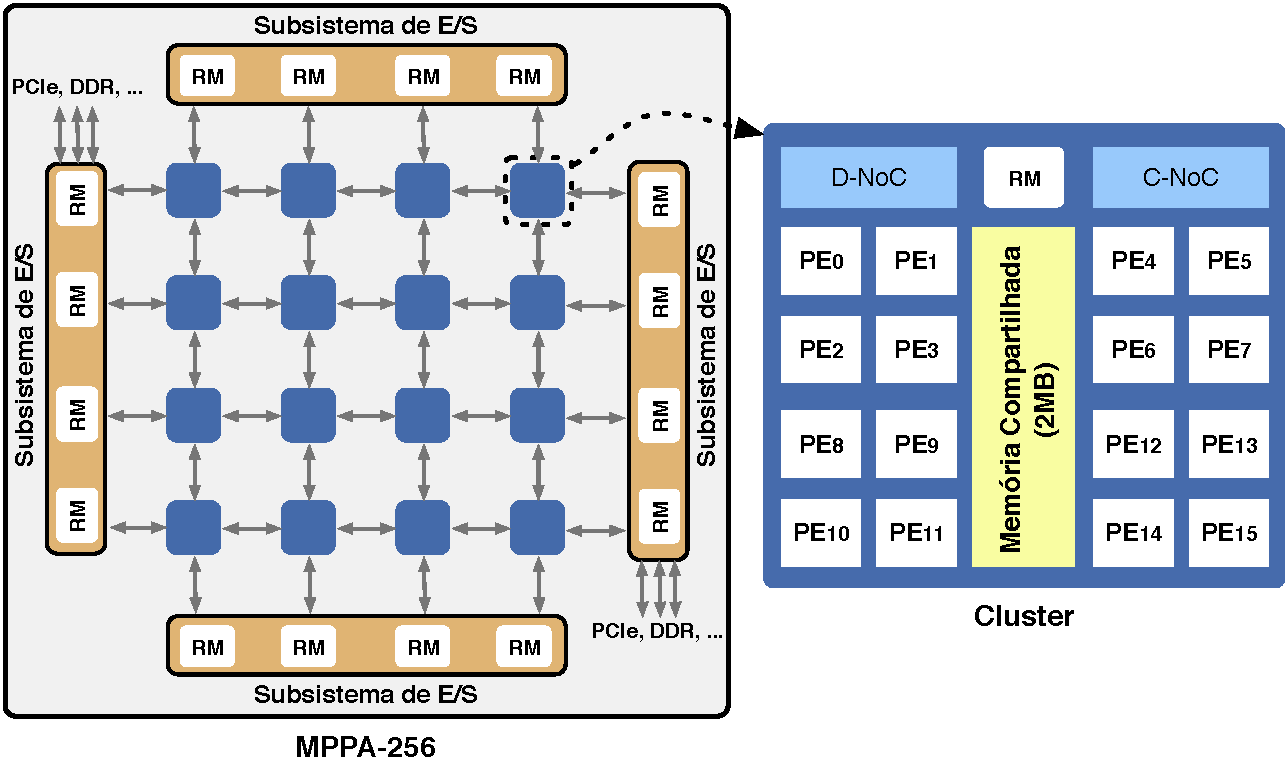
\includegraphics[width=0.75\textwidth]{figs/mppa-overview.pdf} \\
    \legend{Fonte: \cite{castro2013}}
    \label{fig:mppaOverall}
\end{figure}

O processador apresenta um modelo de memória distribuída. Os \clusters de computação e os \clusters de \io possuem espaço de endereçamento próprio. A exploração da computação paralela 
é realizada através de, bibliotecas de código aberto POSIX Threads (Pthreads) e OpenMP, e bibliotecas proprietárias, uma de baixo nível similar a POSIX \ipc e a \async, uma nova biblioteca disponibilizada pela Kalray e desenvolvida a partir da \ipc. As primeiras visam o paralelismo de computação nos \clusters de computação através de memória compartilhada. Enquanto as últimas seguem o modelo de memória distribuída e devem ser usadas para comunicação \cluster--\cluster e \cluster--\io via \noc.

A \async é baseada em comunicação unilateral entre a memória local dos \clusters de computação e a \lpddr. Os principais conceitos por trás da \async são domínios de execução, segmentos e operações de escrita e leitura. O domínio de execução representa um conjuntos de núcleos compartilhando uma memória local, estando isolados de outros domínios de execução. Considerando o modelo de memória distribuída do \mppa, um domínio de execução corresponde a um \cluster de computação ou a um \cluster de \io. Memória que não é acessível diretamente a partir dos núcleos de um domínio de execução pode ser estruturada em segmentos, que correspondem a toda ou parte da memória local de núcleos localizados em outro domínio de execução. Cada segmento tem uma assinatura única, que é especificada quando o segmento é criado em um domínio de execução através da função \texttt{mppa\_async\_segment\_create()}. Então, outros domínios de execução podem referenciar um segmento previamente criado, fornecendo a assinatura única para a função \texttt{mppa\_async\_segment\_clone()}. Assim que segmentos são criados e referenciados por diferentes domínios de execução, eles podem realizar operações de escrita de dados da memória local para um segmento remoto, ou leitura de um segmento remoto para a memória local.
Diferentes funções para realizar estas operações estão disponíveis na biblioteca \async, permitindo transferências de dados contíguos ou espaçados (por exemplo, \texttt{mppa\_async\_put()} e \texttt{mppa\_async\_get\_spaced()}), assim como transferências de blocos 2D (\texttt{mppa\_async\_sget\_block2d()}), que são úteis para transferir dados armazenados em estruturas bidimensionais.

O fluxo de execução de uma aplicação no \mppa ocorre da seguinte maneira: o processo principal (chamado processo mestre) executa em um \rman do \cluster de \io conectado à \lpddr e é responsável por alocar o dado de entrada na sua memória local (\lpddr) e inicializar os processos trabalhadores (uma para cada \cluster de computação) através da função \texttt{mppa\_power\_base\_spawn()}. Os segmentos de dados necessários devem ser criados pelo processo mestre para que a transferência de dados com os \clusters de computação aconteça. Por fim, o processo mestre deve esperar todos os trabalhadores terminarem através da função \texttt{mppa\_power\_base\_waitpid()}. Cada processo trabalhador deve referenciar o segmento remoto criado na \lpddr para realizar leitura e escrita de dados durante a execução, e pode criar até 16 \threads utilizando Pthread ou OpenMP (uma \thread para cada \pe) para computar paralelamente. Cada \pe tem sua \cache de memória privada sem qualquer mecanismo de coerência automático entre as outras \caches de memória dos \pes restantes. Embora isso melhore o desempenho da \cache, é necessário que o desenvolvedor realize o \textit{flush} explícito dos dados quando necessário. 

A biblioteca \ipc e seus detalhes serão retratados na \autoref{sec:pskel-mppa}, que aborda a atual implementação do \pskelmppa, que faz uso desta biblioteca.

Trabalhos anteriores mostraram que desenvolver aplicações paralelas otimizadas para o \mppa é um grande desafio~\cite{francesquini:hal-01092325} devido a alguns fatores importantes, tais como: o modelo de memória distribuída presente no \mppa, a capacidade de memória dentro do \textit{chip} e a comunicação explícita através da \noc. \textit{Podestá Jr.} \etal\cite{wscad2017} apresentam mais detalhes sobre esses desafios.


\section{Esqueletos paralelos}
\label{sec:esqueletosparalelos}

Um esqueleto paralelo é responsável por abstrair um determinado padrão de computação paralela. Para utilizar um esqueleto, o programador definirá as operações principais a serem realizadas, ou seja, definirá o \textit{kernel} da computação. Esse esqueleto será responsável em compor essa função definida pelo usuário, devendo ser executada de maneira correta, paralela e o mais eficiente possível.

A abstração de padrões paralelos contribui para a simplificação e desenvolvimento, além de reduzir o custo de modelagem, facilitar a transformação e otimização das computações.

Devido ao alto nível de abstração, esqueletos paralelos possuem alta afinidade com conceitos presentes nas linguagens de programação, como \textit{templates} e \textit{generics} da linguagem de programação orientada a objetos. Assim, os esqueletos paralelos exploram estes mecanismos \cite{Gorlatch2011}.

\subsection{Padrão estêncil}
\label{subsec:stencil}

Dentre os padrões presentes na literatura, o padrão estêncil é muito utilizado devido a sua aplicação nos campos de simulações meteorológicas, comportamento de fluídos físicos, entre outros.

Ilustrado pela Figura~\ref{fig:stencil}, funciona da seguinte forma: para cada elemento de uma estrutura $n$-dimensional é computado um novo valor relativo aos vizinhos do elemento atual. Os vizinhos de um elemento são determinados pela máscara da computação. Por fim, cada novo valor computado é atribuído à sua célula respectiva em uma estrutura $n$-dimensional de saída. Em aplicações estêncil iterativas, a estrutura de saída é utilizada como estrutura de entrada de uma nova iteração da aplicação.

\begin{figure}
    \centering
    \caption{O padrão estêncil.}
    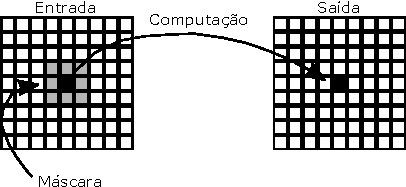
\includegraphics[width=0.75\textwidth]{figs/stencilComputation.pdf} \\
    \legend{Fonte: \cite{wscad2017}}
    \label{fig:stencil}
\end{figure}

\section{\pskel}

O \pskel é um \fw de programação em alto nível para aplicações baseadas no
padrão estêncil, baseado no conceito de esqueletos paralelos, oferecendo suporte para a execução dessas aplicações em
ambientes heterogêneos, incluindo \cpu e \gpu. \pskel oferece um interface única de programação, desacoplada do \textit{back-end} de execução, permitindo que o usuário se preocupe apenas em implementar o \textit{kernel} estêncil que descreve a computação, enquanto o \fw fica responsável pela tradução das abstrações descritas para código paralelo de baixo nível em C++, gestão de memória e transferência de dados. Tudo isso de forma transparente para o usuário~\cite{CPE:CPE3479}.

O \autoref{code:pskel} mostra um exemplo do método Jacobi para resolver equações matriciais~\cite{demmel97} com o \pskel. A \api do \pskel fornece estruturas genéricas para manipular os dados de entrada e saída, chamadas \texttt{Array}, \texttt{Array2D} (\autoref{code:pskel}, linhas 12--13) e \texttt{Array3D}, através do uso de \textit{templates} da linguagem de programação C++. Essas abstrações fornecem métodos que encapsulam o gerenciamento dos dados, como alocação de memória, cópia de memória e transferência de dados entre \cpu e \gpu. Além disso, fornece abstrações para definição da computação estêncil e gerenciamento de sua execução. A computação estêncil é definida na função \texttt{stencilKernel()} (\autoref{code:pskel}, linhas 1--3), ela deve ser implementada pelo usuário do \pskel, é o método específico de cada aplicação, o qual descreve como a computação será realizada sobre cada elemento da matriz de entrada e seus vizinhos. O conjunto de classes para gerenciamento da execução são \texttt{Stencil}, \texttt{Stencil2D} (\autoref{code:pskel}, linha 15) e \texttt{Stencil3D}.

No exemplo fornecido, a função \texttt{stencilKernel()} será executada na GPU. O método \texttt{runIterativeGPU()} livra o usuário de escrever código específico na linguagem CUDA, necessário para excutar corretamente a computação estêncil na \gpu.

\begin{figure}
\begin{lstlisting}[
    caption={Trecho simplificado de código estêncil com \pskel.}, 
    label=code:pskel,
    language=C++,
    keywordstyle=\color{blue}\bfseries,
    otherkeywords = {__parallel__,struct,Array2D,Stencil2D}, 
    basicstyle=\tiny, 
    frame = single,]
__parallel__ void
stencilKernel(Array2D<float> A, Array2D<float> B, 
              struct Arguments args, int x, int y) {

    B(x,y) = args.alpha * (A(x,y+1) + A(x,y-1) + A(x+1,y) + A(x-1,y) 
             + args.beta);
}
        
void jacobi(float *A, float *B, int M, int N, float alpha, 
            float beta, int timesteps) {

    Array2D<float> input(A,M,N);
    Array2D<float> output(B,M,N);
    struct Arguments args(alpha, beta);
    Stencil2D<Array2D<float>, struct Arguments> stencil(input,output,args);
    stencil.runIterativeGPU(timesteps);
}
\end{lstlisting}
\end{figure}

\section{PSkel-MPPA}
\label{sec:pskel-mppa}

A adaptação PSkel-MPPA, é uma adaptação do \pskel proposta por~\cite{wscad2017}, ela faz uso de uma \api similar à POSIX \ipc para comunicação e será tratada como \ipc no decorrer deste trabalho. Nela, são utilizados portais de comunicação para o envio de dados e o método de \textit{strides}  para gerenciar explicitamente o envio e recebimento de \textit{tiles}.

\begin{figure}
    \centering
    \caption{Esquemático da proposta \pskelmppa.}
    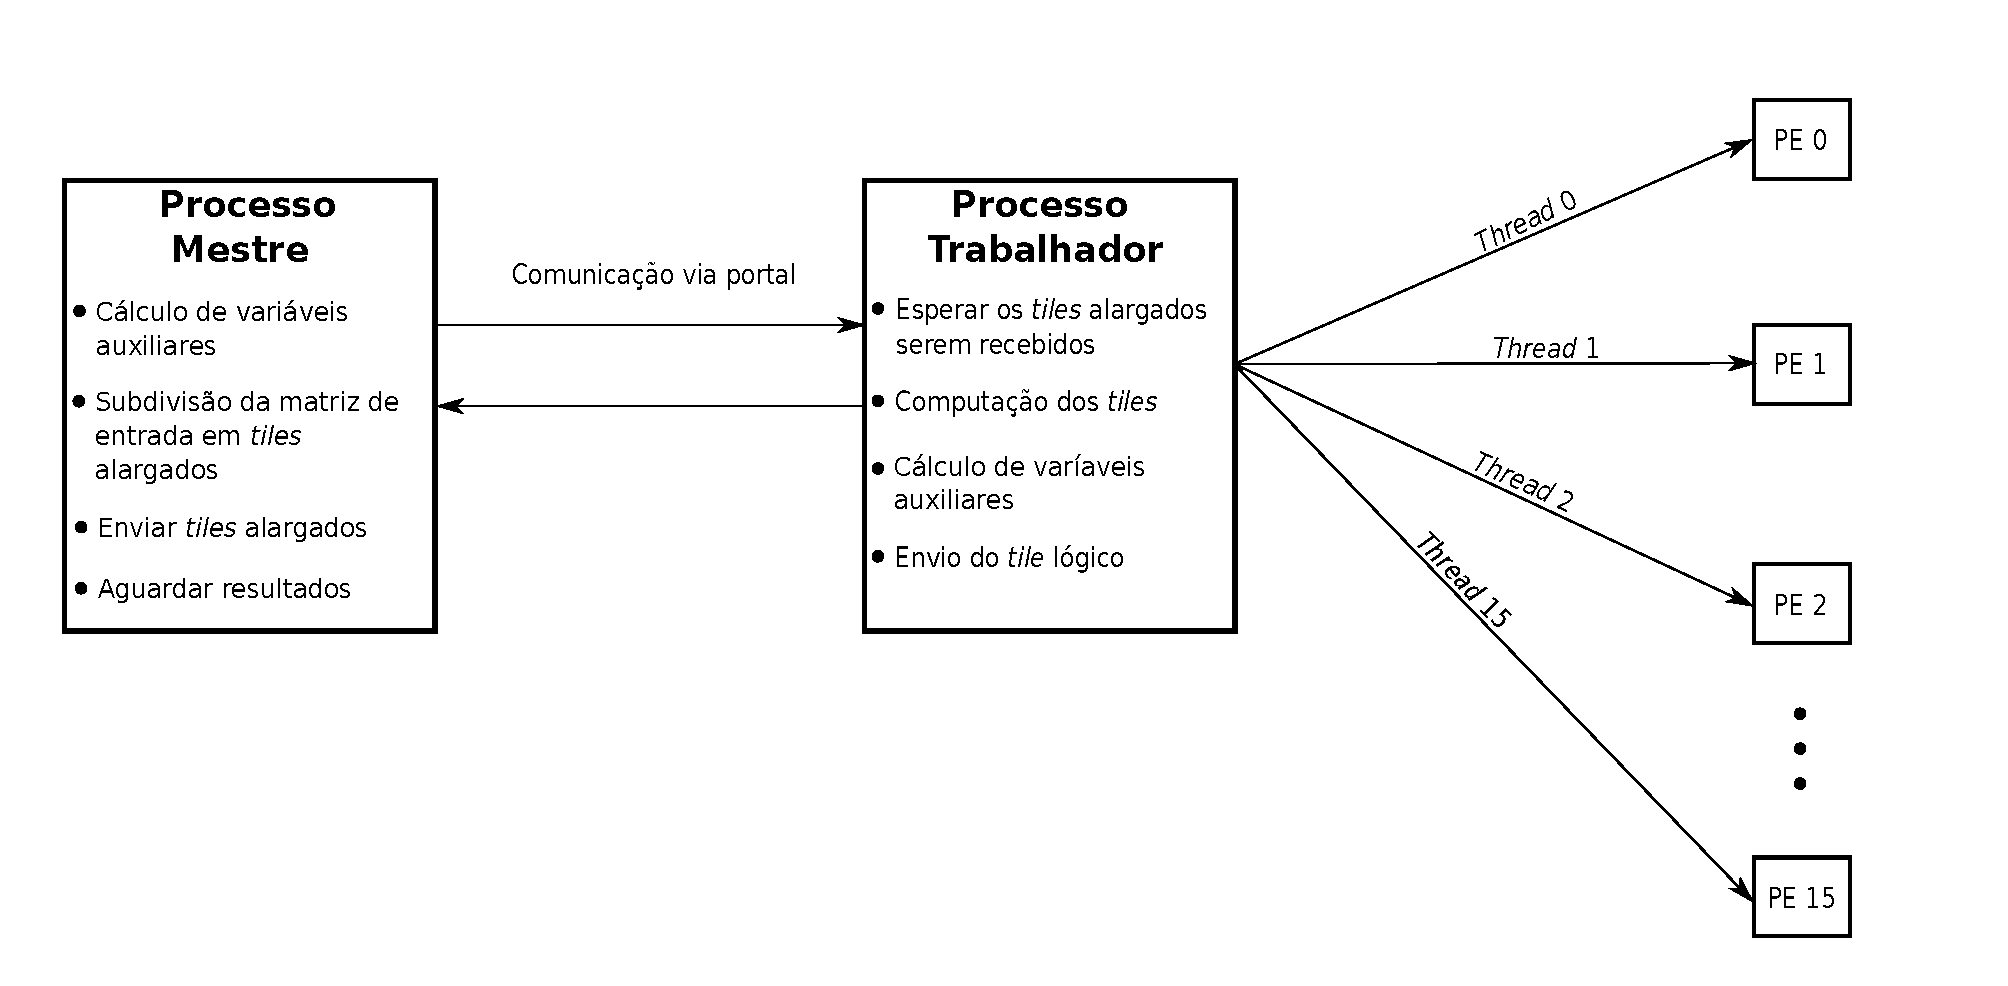
\includegraphics[width=1\textwidth]{figs/visaoGeralPSKELMPPATrabalhador.pdf} \\
    \legend{Fonte - {\cite{Podesta:TCC}}}
    \label{fig:visaoGeralPSkelMPPA}
\end{figure}


A Figura~\ref{fig:visaoGeralPSkelMPPA} ilustra a adaptação
desenvolvida. É empregado o modelo mestre-trabalhador, que é um dos padrões de computação paralela utilizado quando existem múltiplos núcleos de processamento. O processo mestre é executado no \cluster de \io conectado a memória LPDDR3, aonde os dados de entrada e saída (os \emph{Array2Ds}) são alocados. Em seguida, ele calcula o número de \tiles alargados que serão produzidos, assim como suas dimensões baseado em: i) parametros definidos pelo usuário, como o tamanho da entrada de dados e as dimensões do \tile lógico, o número de \emph{clusters} de computação e o número de iterações internas; e ii) parâmetros do \emph{kernel} estêncil, como o tamanho da máscara. Então, são lançados até 16 processos trabalhadores (um em cada \cluster de computação) e é informado a cada processo trabalhador, o \tile pelo qual será responsável por processar na atual iteração. Cada processo trabalhador, por outro lado, aloca dados para armazenar o \tile alargado de entrada e de saída na memória local do \cluster de computação.

A fase de computação consiste da execução do \emph{kernel} estêncil pelos processos trabalhadores. As seguintes três principais etapas são realizadas para computar cada \tile atribuído a um processo trabalhador: 1) o \tile alargado é extraido do dado de entrada alocado na \lpddr e transferido para a memória local do \cluster de computação para ser processado, a extração e transferência é realizada com o uso de portais; 2) $t^\prime$ iterações do \emph{kernel} estêncil (iterações internas) são executadas pelo processo trabalhor sobre o \tile alargado, sincronizando com o processo mestre ao final das iterações internas, com o objetivo de receber um novo \textit{tile} ou para preparação dos dados a serem computados pelos trabalhadores nas iterações seguintes, ou término da execução; e 3). Ao alcançar o número total de iterações ($t$) definido pelo usuário, estará presente na \lpddr o \textit{Array2D} computado.

A comunicação realizada entre os processos mestre e trabalhadores é realizada por meio de portais, provenientes de uma \api proprietária de baixo nível do \mppa, similar à POSIX IPC. Os portais são responsáveis por realizar escrita e leitura de maneira remota, para isso um processo que deseja comunicar-se deve criar um portal com uma classificação (\textit{tag}) e relacioná-lo a um espaço de endereçamento, para posteriormente realizar leitura ou escrita no endereço associado.

A memória nos \textit{clusters} de computação (2MB) é limitada, devido a isso a matriz de entrada da computação (\textit{Array2D}) é particionada em tamanhos menores denominados \textit{tiles}, que possuem tamanho fixo definido pelo usuário para serem enviados aos \textit{clusters}.

As operações sobre \textit{tiles} e matrizes são realizadas sobre endereços de memória. Devido a restrição da \api e da \noc no \mppa, os dados armazenados em cada \textit{tile} precisam estar contíguos em memória para serem transferidos
pela \noc. Com o objetivo de evitar cópias locais de dados, utiliza-se o conceito de \textit{strides}. Cada \textit{stride} é uma parte contígua do \texttt{Array} original, sendo determinado por deslocamentos (\textit{offsets}) especificados durante a
execução. Os deslocamentos são dinâmicos e dependem dos \textit{tiles} sendo computados. Essas informações são conhecidas pelo processo mestre por meio da utilização da classe \texttt{StencilTiling}, e este as repassa aos processos trabalhadores \cite{Podesta:TCC}.

\begin{figure}[t]
	\centering
    \caption{Exemplo do funcionamento do método \textit{strides} no \mppa.}
	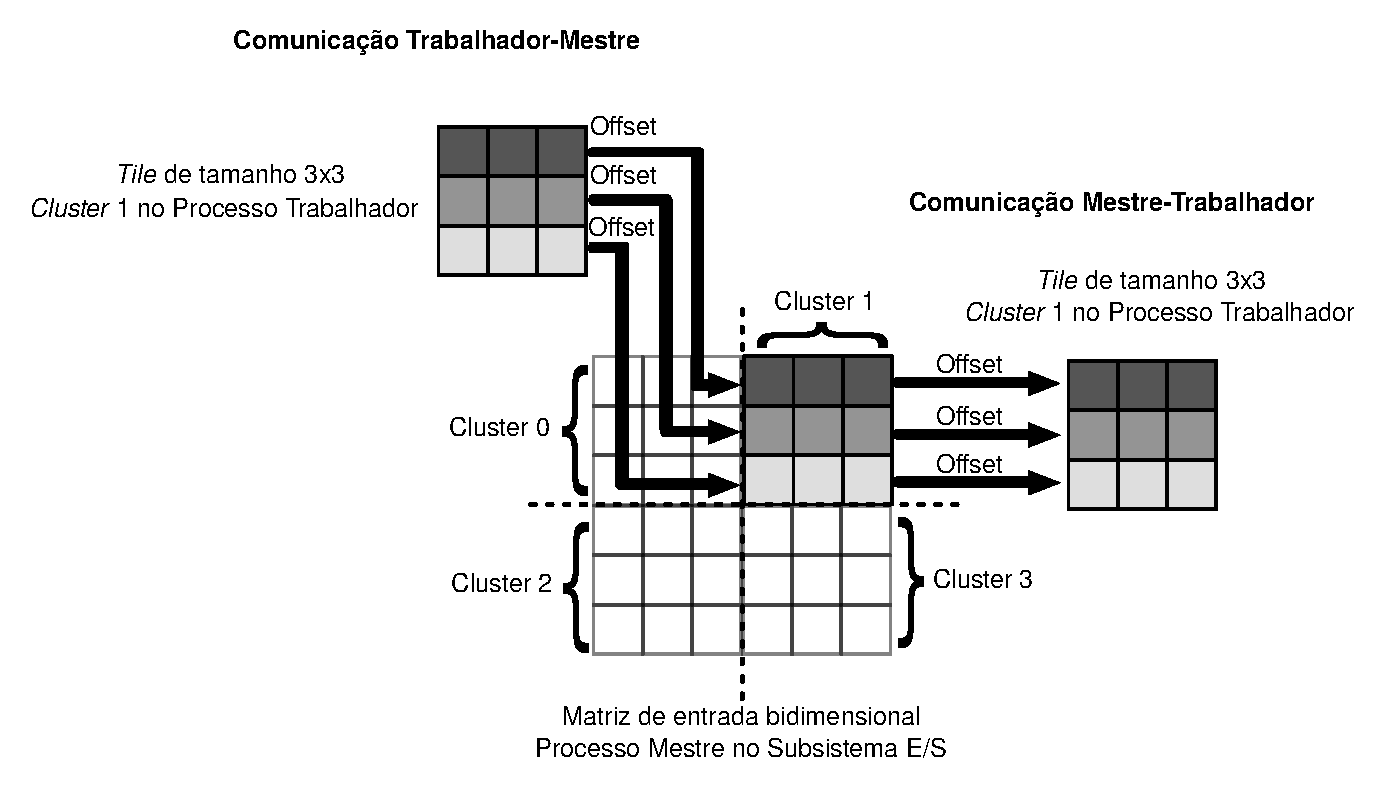
\includegraphics[width=0.9\textwidth]{figs/stridesImage.pdf} \\
    \legend{Fonte: {\cite{Podesta:TCC}}}
	\label{fig:strides}
\end{figure}


A Figura~\ref{fig:strides} ilustra o processo de comunicação com o método \textit{strides} para o caso de uma matriz de entrada de tamanho 6x6, \textit{tiles} de tamanho 3x3 e 4 \textit{clusters}. Ao computar todos os deslocamentos, o método irá enviar diretamente, via portal, os dados especificados pelo endereço inicial do \textit{tile} e pelos saltos na memória com a área útil especificada. Com isso, é possível enviar de forma contígua e direta os \textit{tiles} a outro processo, sem a necessidade de cópias locais \cite{Podesta:TCC}.

Quando se trata de particionamento de computação estêncil, é necessário tratar as depedências de vizinhança provenientes do padrão paralelo estêncil, antes de particionar os dados de entrada. A técnica de \textit{tiling} trapezoidal é utilizada para tratar as dependências de vizinhança, o que resulta na computação e presença redundante de dados~\cite{Rocha:2017}, porém em troca da presença de computação e dados redundantes, se reduz a quantidade de comunicações e sincronizações necessárias a serem realizadas, que se mostram extremamente prejudiciais para o desempenho. A definição formal está ilustrada a seguir.
Seja $A$ uma matriz de dados 2D, com dimensões $\textrm{dim}(A) = (w, h)$, aonde $w$ e $h$ são, respectivamente, sua largura e altura.
Utilizando \tiles de dimensões $(w^\prime, h^\prime)$ temos $\lceil\frac{w}{w^\prime}\rceil\lceil\frac{h}{h^\prime}\rceil$ como sendo os possíves \tiles de $A$.
Seja $A_{i,j}$ um único \tile, onde $0\leq i < \lceil\frac{w}{ w^\prime}\rceil$ e $0\leq j < \lceil\frac{h}{ h^\prime}\rceil$.
$A_{i,j}$ possui um deslocamento de $(i w^\prime,j h^\prime)$ em relação ao canto superior esquerdo de $A$ e $\textrm{dim}(A_{i,j}) = (\min\{w^\prime, w-i w^\prime\}, \min\{h^\prime, h-j h^\prime\})$.
Esse deslocamento atua como um indexador necessário para acessar os elementos de um \tile.

A Figura~\ref{fig:gputile} mostra a representação gráfica dessa técnica. Um \tile lógico (linha contínua interna) está contido em uma matriz de dados 2D (linha pontilhada externa) com deslocamento vertical e horizontal definidos por $j h^\prime$ e $i w^\prime$. Se $t$ iterações de uma aplicação estêncil devem ser executadas, é possível computar $t^\prime$ consecutivas iterações em $A_{i,j}$ ($t^\prime \in \left[1,t\right]$) se precissar de qualquer troca de dados entre \tiles adjacentes (também conheçido como iterações internas). Assim, o \tile lógico ($A_{i,j}$) precisa ser alargado, com o acréscimo de uma \emph{ghost zone} (área entre a linha sólida interna e externa), o que inclui a \emph{halo region} (a área entre a linha sólida interna e a linha pontilhada interna). Seja $r$ o mais distante deslocamento necessário para a vizinhança definida pela máscara estêncil. A área de alcance $r$ que define a vizinhança é denominada \textit{halo region}. O número de \emph{halo regions} adjacentes que compõe a \emph{ghost zone} é proporcional a $t^\prime$.
%
Assim, \tile alargado $A^\ast_{i,j}$ possui deslocamentos $(\max\{iw^\prime - rt^\prime, 0\}, \max\{jh^\prime - rt^\prime, 0\})$ relativos a $A$ \cite{Podesta:TCC}. 

\begin{figure}
	\centering
	\caption{Técnica de \textit{tiling} 2D.}
	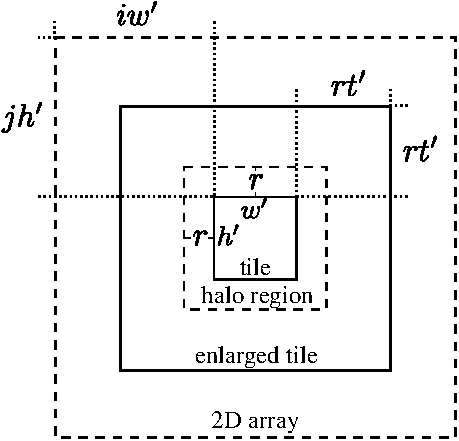
\includegraphics[width=0.5\textwidth]{figs/tile.pdf} \\
	\legend{Fonte: {\cite{Rocha:2017}}}
	\label{fig:gputile}
\end{figure}

Felizmente, todas a complexas tarefas relacionas a técnica de \textit{tiling}, comunicação via \noc e adaptações discutidas nessa seção são transparentes para o usuário, tendo em vista que estão incluidas no \emph{back-end} do PSkelMPPA.


    % Capitulo de revisão de literatura
    % The \phantomsection command is needed to create a link to a place in the document that is not a
% figure, equation, table, section, subsection, chapter, etc.
%
% When do I need to invoke \phantomsection?
% https://tex.stackexchange.com/questions/44088/when-do-i-need-to-invoke-phantomsection
\phantomsection
\chapter{Trabalhos Relacionados}
\phantomsection

Devido a importância dos esqueletos paralelos, e especifcamente o padrão paralelo estêncil, muitos esforços de pesquisas recentes buscam melhorar o desempenho e o suporte desses esqueletos em processadores manycore. \textit{Buono} \etal\cite{buono13} portaram um \fw baseado em esqueletos paralelos, chamado \textit{FastFlow}, para o processador \textit{manycore} TilePro64, que possui 64 núcleos de processamento idênticos, interconectados por uma malha de \noc. Similarmente, \textit{Thorarensen} \etal\cite{thoraransen16} apresentaram um novo \textit{back-end} do \fw SkePU para o processador \textit{manycore} Myriad2. Que possui como característica uma arquitetura heterogênea, visando dispositivos com restrição de energia e principalmente aplicações de visão computacional. \textit{Gysi} \etal\cite{gysi15} propuseram um \fw para otimização automática da repartição de computações estêncil em sistemas híbridos de \cpu e \gpu.

Recentes trabalhos estudaram o desempenho e/ou a eficiência energética de processadores manycore de baixa potência. \textit{Totoni} \etal\cite{SCCEnergy:2012} compararam a potência e o desempenho do \textit{Intel's Single-Chip Cloud Computer} (SCC) com outros tipos de \textit{CPUs} e \textit{GPUs}. Porém, eles mostraram que não existe um solução única que entrega o melhor troca entre potência e performance, os resultados mostram que \textit{manycores} são uma oportunidade para o futuro. \textit{Souza} \etal\cite{Castro-Souza-CCPE:2016} propuseram um conjunto de \textit{benchmarks} para avaliar o \mppa manycore processor. O \textit{benchmark} oferece diversas aplicações que utilizam padrões paralelos, tipos de trabalho, intensidade de comunicação e estratégias de carga de trabalho, adequado para uma ampla compreensão do desempenho e consumo de energia do \mppa e novos \textit{manycores} que estão por vir. \textit{Francesquini} \etal\cite{francesquini:hal-01092325} avaliaram três diferentes classes de aplicação (consumo de CPU, consumo de memória e uma composição híbrida dos dois tipos anteriores) utilizando plataformas de alto paralelismo como o \mppa em uma plataforma NUMA de 24 nós e 192 núcleos. Eles mostraram que as arquiteturas \textit{manycore} podem ser competitivas, mesmo se a aplicação é irregular por natureza.

De acordo com relevante conhecimento na área, o \pskelmppa é a primeira implementação completa de um \fw com uso de padrões paralelos no \mppa. A solução proposta livra os programadores da necessidade de lidar explicitamente com a gestão de comunicação e envio de dados pela \noc, assim como a preocupação de lidar com um ambiente híbrido de execução e a ausência de coerência de \textit{cache} no \mppa.

    % Capitulo de Desenvolvimento
    % The \phantomsection command is needed to create a link to a place in the document that is not a
% figure, equation, table, section, subsection, chapter, etc.
%
% When do I need to invoke \phantomsection?
% https://tex.stackexchange.com/questions/44088/when-do-i-need-to-invoke-phantomsection
\phantomsection

% ---
\chapter{Otimização PSkel-MPPA}
\phantomsection





    % Capitulo de Resultados
    % The \phantomsection command is needed to create a link to a place in the document that is not a
% figure, equation, table, section, subsection, chapter, etc.
%
% When do I need to invoke \phantomsection?
% https://tex.stackexchange.com/questions/44088/when-do-i-need-to-invoke-phantomsection
\phantomsection

% ---
\chapter{Experimentos}
\phantomsection

    
    
    
    % Finaliza a parte no bookmark do PDF
    % para que se inicie o bookmark na raiz
    % e adiciona espaço de parte no Sumário
    \phantompart
    
    % Conclusão (outro exemplo de capítulo sem numeração e presente no sumário)
    % The \phantomsection command is needed to create a link to a place in the document that is not a
% figure, equation, table, section, subsection, chapter, etc.
%
% When do I need to invoke \phantomsection?
% https://tex.stackexchange.com/questions/44088/when-do-i-need-to-invoke-phantomsection
\phantomsection

% ---
\chapter{Conclusão}
\label{cap:conclusao}
\phantomsection

\todo[inline]{Descreva a conclusão do que foi apresentado no TCC I.}

% O desenvolvimento de aplicações otimizadas para processadores \textit{manycore} de baixa potência é bastante desafiador devido a fatores importantes tais como a existência de um modelo de programação híbrido, capacidade limitada de memória no \textit{chip}, ausência de coerência de \textit{cache}, entre outros. Neste artigo foi apresentada uma nova versão otimizada do \fw \pskel para o processador \mppa. Os resultados mostraram que a nova versão obteve ganhos de desempenho de até $8$x e uma redução no consumo de energia de até $6$x, em comparação com a solução inicial proposta em~\cite{wscad2017}. Como trabalhos futuros, pretende-se comparar o desempenho e consumo de energia com outros processadores e implementar suporte a matrizes tridimensionais.



    % ELEMENTOS PÓS-TEXTUAIS
    \postextual
    \setlength\beforechapskip{0pt}
    \setlength\midchapskip{15pt}
    \setlength\afterchapskip{15pt}

    % Referências bibliográficas
    \begingroup
        % Using BibTeX to make a list of references without having citations in the body of the document?
        % https://tex.stackexchange.com/questions/17128/using-bibtex-to-make-a-list-of-references-without
        % \nocite{*}

        \printbibliography[title=REFERÊNCIAS]
    \endgroup

    % Glossário, consulte o manual da classe abntex2 para orientações sobre o glossário.
    % \ifforcedinclude\else\glossary\fi

    % Apêndices, inicia os apêndices
    \begin{apendicesenv}
        % Imprime uma página indicando o início dos apêndices
        \ifforcedinclude\else\partapendices\fi

        \setlength\beforechapskip{50pt}
        \setlength\midchapskip{20pt}
        \setlength\afterchapskip{20pt}

        % %
% How to fix the Underfull \vbox badness has occurred while \output is active on my memoir chapter style?
% https://tex.stackexchange.com/questions/387881/how-to-fix-the-underfull-vbox-badness-has-occurred-while-output-is-active-on-m
%

% ---

\lang
{\chapter[Page not filled]{Since this page is not being completely filled, it is generating the bottom bottom of the page}}
{\chapter[Página não gerada]{Como esta página não está sendo completamente preenchida, ele está gerando a caixa inferior inferior da página}}
% ---


% Multiple-language document - babel - selectlanguage vs begin/end{otherlanguage}
% https://tex.stackexchange.com/questions/36526/multiple-language-document-babel-selectlanguage-vs-begin-endotherlanguage
\begin{otherlanguage*}{english}

 

1. How to display the font size in use in the final output,
2. How to display the font size in use in the final output,
3. How to display the font size in use in the final output,
4. How to display the font size in use in the final output,
5. How to display the font size in use in the final output,
6. How to display the font size in use in the final output,
7. How to display the font size in use in the final output,
8. How to display the font size in use in the final output,
9. How to display the font size in use in the final output,


% As this page is not being completely filled, it is generating the page bottom bad box.
% Fix Underfull \vbox (badness 10000) has occurred while \output is active
%
% \flushbottom vs \raggedbottom
% https://tex.stackexchange.com/questions/65355/flushbottom-vs-raggedbottom
\newpage



\section[Some encoding tests]{ }

1. How to display the font size in use in the final output,
2. How to display the font size in use in the final output,
3. How to display the font size in use in the final output,
4. How to display the font size in use in the final output,
5. How to display the font size in use in the final output,
6. How to display the font size in use in the final output,

7. How to display the font size in use in the final output,
8. How to display the font size in use in the final output,
9. How to display the font size in use in the final output,
10. How to display the font size in use in the final output,
11. How to display the font size in use in the final output,
12. How to display the font size in use in the final output,

\subsection{ }

1. How to display the font size in use in the final output,
2. How to display the font size in use in the final output,
3. How to display the font size in use in the final output,
4. How to display the font size in use in the final output,
5. How to display the font size in use in the final output,
6. How to display the font size in use in the final output,

7. How to display the font size in use in the final output,
8. How to display the font size in use in the final output,
9. How to display the font size in use in the final output,
10. How to display the font size in use in the final output,
11. How to display the font size in use in the final output,
12. How to display the font size in use in the final output,

\subsubsection{ }

1. How to display the font size in use in the final output,
2. How to display the font size in use in the final output,
3. How to display the font size in use in the final output,
4. How to display the font size in use in the final output,
5. How to display the font size in use in the final output,
6. How to display the font size in use in the final output,

7. How to display the font size in use in the final output,
8. How to display the font size in use in the final output,
9. How to display the font size in use in the final output,
10. How to display the font size in use in the final output,
11. How to display the font size in use in the final output,
12. How to display the font size in use in the final output,

\subsubsubsection{ }

1. How to display the font size in use in the final output,
2. How to display the font size in use in the final output,
3. How to display the font size in use in the final output,
4. How to display the font size in use in the final output,
5. How to display the font size in use in the final output,
6. How to display the font size in use in the final output,
7. How to display the font size in use in the final output,

8. How to display the font size in use in the final output,
9. How to display the font size in use in the final output,
10. How to display the font size in use in the final output,
11. How to display the font size in use in the final output,
12. How to display the font size in use in the final output,


Lipsum me [31-35]

\end{otherlanguage*}



    \end{apendicesenv}

    % Anexos, inicia os anexos
    \begin{anexosenv}
        % Imprime uma página indicando o início dos anexos
        \ifforcedinclude\else\partanexos\fi

        \setlength\beforechapskip{50pt}
        \setlength\midchapskip{20pt}
        \setlength\afterchapskip{20pt}

        % %
% How to fix the Underfull \vbox badness has occurred while \output is active on my memoir chapter style?
% https://tex.stackexchange.com/questions/387881/how-to-fix-the-underfull-vbox-badness-has-occurred-while-output-is-active-on-m
%

% ----------------------------------------------------------
\chapter{\lang{Article published in SOBRAEP magazine}{Artigo publicado}}
% ----------------------------------------------------------


% Multiple-language document - babel - selectlanguage vs begin/end{otherlanguage}
% https://tex.stackexchange.com/questions/36526/multiple-language-document-babel-selectlanguage-vs-begin-endotherlanguage
\begin{otherlanguage*}{english}

% An environment for setting \emergencystretch locally
% https://tex.stackexchange.com/questions/84510/an-environment-for-setting-emergencystretch-locally
{
    \setlength{\emergencystretch}{10pt}
    \section[English guidelines for publication]
    {English guidelines for publication - TITLE HERE (14 PT TYPE SIZE, UPPERCASE, BOLD, CENTERED)}
}
    \noindent\textbf{Abstract:}
    The objective of this document is to instruct the authors about the preparation of the
    manuscript for its submission to the Revista Eletrônica de Potência (Brazilian Power Electronics
    Journal).~The authors should use these guidelines for preparing both the initial and final
    versions of their paper. Additional information about procedures and guidelines for publication
    can be obtained directly with the editor, or through the web site
    \url{http://www.sobraep.org.br/revista}. This text was written according to these guidelines

\end{otherlanguage*}

% What is a “Overfull \hbox (9.89561pt too wide)”?
% https://tex.stackexchange.com/questions/111948/what-is-a-overfull-hbox-9-89561pt-too-wide
interwordspace: \the\fontdimen2\font

interwordstretch: \the\fontdimen3\font

emergencystretch: \the\emergencystretch\par\relax


\modifiedincludepdf{-}{ArtigoSOBRAEP}{pictures/SOBRAEP.pdf}{0.9}



        % %
% How to fix the Underfull \vbox badness has occurred while \output is active on my memoir chapter style?
% https://tex.stackexchange.com/questions/387881/how-to-fix-the-underfull-vbox-badness-has-occurred-while-output-is-active-on-m
%

% ----------------------------------------------------------
\lang
{\chapter[Sample example]{How to display the font size in use in the final output}}
{\chapter[Anexo exemplo]{Como exibir o tamanho da fonte em uso na saída final}}
% ----------------------------------------------------------


% Multiple-language document - babel - selectlanguage vs begin/end{otherlanguage}
% https://tex.stackexchange.com/questions/36526/multiple-language-document-babel-selectlanguage-vs-begin-endotherlanguage
\begin{otherlanguage*}{english}

 

1. How to display the font size in use in the final output,
2. How to display the font size in use in the final output,
3. How to display the font size in use in the final output,


\section[Some encoding tests]{ }

1. How to display the font size in use in the final output,
2. How to display the font size in use in the final output,
3. How to display the font size in use in the final output,
4. How to display the font size in use in the final output,
5. How to display the font size in use in the final output,
6. How to display the font size in use in the final output,

7. How to display the font size in use in the final output,
8. How to display the font size in use in the final output,
9. How to display the font size in use in the final output,
10. How to display the font size in use in the final output,
11. How to display the font size in use in the final output,
12. How to display the font size in use in the final output,

\subsection{ }

1. How to display the font size in use in the final output,
2. How to display the font size in use in the final output,
3. How to display the font size in use in the final output,
4. How to display the font size in use in the final output,
5. How to display the font size in use in the final output,
6. How to display the font size in use in the final output,

7. How to display the font size in use in the final output,
8. How to display the font size in use in the final output,
9. How to display the font size in use in the final output,
10. How to display the font size in use in the final output,
11. How to display the font size in use in the final output,
12. How to display the font size in use in the final output,

\subsubsection{ }

1. How to display the font size in use in the final output,
2. How to display the font size in use in the final output,
3. How to display the font size in use in the final output,
4. How to display the font size in use in the final output,
5. How to display the font size in use in the final output,
6. How to display the font size in use in the final output,

7. How to display the font size in use in the final output,
8. How to display the font size in use in the final output,
9. How to display the font size in use in the final output,
10. How to display the font size in use in the final output,
11. How to display the font size in use in the final output,
12. How to display the font size in use in the final output,

\subsubsubsection{ }

1. How to display the font size in use in the final output,
2. How to display the font size in use in the final output,
3. How to display the font size in use in the final output,
4. How to display the font size in use in the final output,
5. How to display the font size in use in the final output,
6. How to display the font size in use in the final output,
7. How to display the font size in use in the final output,

8. How to display the font size in use in the final output,
9. How to display the font size in use in the final output,
10. How to display the font size in use in the final output,
11. How to display the font size in use in the final output,
12. How to display the font size in use in the final output,


Lipsum me [55-65]

\end{otherlanguage*}



    \end{anexosenv}

    % INDICE REMISSIVO
    \ifforcedinclude\else
        \phantompart
        \printindex
    \fi

\end{document}
